% ============================================================
%  main.tex  —  Root document
%  ML-Based Groundwater Potential Mapping of the Pothohar
%  Plateau, Punjab, Pakistan
%
%  Compile (Overleaf or local):
%     pdflatex main  →  bibtex main  →  pdflatex main  →  pdflatex main
% ============================================================
\documentclass[12pt,a4paper,oneside]{report}

% ============================================================
%  settings.tex  —  Global formatting, packages, and macros
%  ML-Based Groundwater Potential Mapping — Pothohar Plateau
%  Engine: XeLaTeX + BibTeX (IEEEtran)   |   Overleaf-ready
% ============================================================

% ---- Page geometry (A4, bound-thesis margins) --------------
\usepackage[a4paper,left=1.5in,right=1in,top=1in,bottom=1in]{geometry}

% ---- Fonts (XeLaTeX / fontspec) ----------------------------
\usepackage{fontspec}
% Default main font is Latin Modern (always available — no download), so
% the document compiles on a fresh MiKTeX. To use a Times-style font for
% final submission, install the "tex-gyre" package in the MiKTeX Console
% then uncomment the line below:
% \setmainfont{texgyretermes}[Extension=.otf,UprightFont=*-regular,BoldFont=*-bold,ItalicFont=*-italic,BoldItalicFont=*-bolditalic]
\usepackage{microtype}

% ---- Line spacing ------------------------------------------
\usepackage{setspace}
\onehalfspacing                   % 1.5 line spacing (thesis standard)

% ---- Math & units ------------------------------------------
\usepackage{amsmath,amssymb}
% (Math is set in Latin Modern Math, which XeLaTeX supports out of the
%  box. unicode-math is intentionally NOT loaded — it requires a separate
%  OpenType math font and is a common first-build failure point.)
\usepackage{siunitx}              % \SI{25000}{\kilo\meter\squared}
\sisetup{per-mode=symbol,detect-weight=true}

% ---- Tables ------------------------------------------------
\usepackage{booktabs}            % \toprule \midrule \bottomrule
\usepackage{multirow}
\usepackage{array}
\usepackage{longtable}

% ---- Figures -----------------------------------------------
\usepackage{graphicx}
\graphicspath{{figures/}}        % all 52 figures resolve by bare name
\usepackage{float}               % [H] exact float placement
\usepackage{caption}
\usepackage{subcaption}
\captionsetup{font=small,labelfont=bf,justification=centering}

% ---- Colour ------------------------------------------------
\usepackage[dvipsnames,table]{xcolor}

% ---- Bibliography: IEEE numeric [1],[2] --------------------
\usepackage[numbers,square,sort&compress]{natbib}
\bibliographystyle{IEEEtran}

% ---- Hyperlinks (load late) --------------------------------
\usepackage[hidelinks,breaklinks=true]{hyperref}
\hypersetup{
  colorlinks=true,
  linkcolor=black,
  citecolor=NavyBlue,
  urlcolor=NavyBlue,
  pdftitle={ML-Based Groundwater Potential Mapping of the Pothohar Plateau},
  pdfauthor={M.Sc. Thesis, NUST MISIS}
}

% ---- Headers / footers -------------------------------------
\usepackage{fancyhdr}
\pagestyle{fancy}
\fancyhf{}
\renewcommand{\headrulewidth}{0.4pt}
\fancyhead[L]{\nouppercase{\leftmark}}
\fancyhead[R]{\thepage}
\fancypagestyle{plain}{\fancyhf{}\fancyfoot[C]{\thepage}\renewcommand{\headrulewidth}{0pt}}

% ---- Chapter title styling ---------------------------------
\usepackage{titlesec}
\titleformat{\chapter}[display]
  {\normalfont\huge\bfseries}
  {\chaptertitlename\ \thechapter}{12pt}{\Huge}
\titlespacing*{\chapter}{0pt}{0pt}{24pt}

% ---- Lists -------------------------------------------------
\usepackage{enumitem}
\setlist{itemsep=2pt,topsep=3pt}

% ---- Convenience macros ------------------------------------
\newcommand{\studyarea}{Pothohar Plateau}
\newcommand{\npixels}{37{,}015{,}091}


\begin{document}

% ---------------- Front matter (roman numerals) -------------
\pagenumbering{roman}

% ============================================================
%  Title Page
%  >>> FILL IN the [[...]] placeholders before submission <<<
% ============================================================
\begin{titlepage}
\centering
\thispagestyle{empty}

{\scshape\large [[University Name]]\par}
{\scshape [[Department / Faculty Name]]\par}
\vspace{0.8cm}

% --- University logo (optional) ---
% \includegraphics[width=0.25\textwidth]{university_logo}\par
% \vspace{0.6cm}

\vfill
{\Huge\bfseries ML-Based Groundwater Potential Mapping of the Pothohar Plateau, Punjab, Pakistan\par}
\vspace{0.5cm}
{\large A Machine Learning Approach Extending Knowledge-Based Weighted Overlay\par}
\vfill

{\large A thesis submitted in partial fulfillment of the requirements\\
for the degree of\\[0.3cm]
\textbf{[[Master of Science in Data Science / Geographic Information Systems]]}\par}

\vfill
{\large\itshape Submitted by\par}
{\Large\bfseries [[Student Full Name]]\par}
{\large Registration No.: [[Reg. No.]]\par}

\vspace{0.8cm}
{\large\itshape Supervised by\par}
{\Large [[Supervisor Name and Designation]]\par}

\vfill
{\large [[Month, Year]]\par}

\end{titlepage}
\cleardoublepage

% ============================================================
%  Certificate of Approval
% ============================================================
\chapter*{Certificate}
\addcontentsline{toc}{chapter}{Certificate}
\thispagestyle{plain}

\noindent
This is to certify that the thesis entitled \textbf{``ML-Based Groundwater
Potential Mapping of the Pothohar Plateau, Punjab, Pakistan''} submitted by
\textbf{[[Student Full Name]]} (Registration No. [[Reg. No.]]) has been
carried out under my supervision and is approved for submission in partial
fulfillment of the requirements for the degree of \textbf{[[Degree]]} at
\textbf{[[University Name]]}.

\vspace{2cm}

\noindent
\begin{minipage}{0.5\textwidth}
\centering
\rule{6cm}{0.4pt}\\
\textbf{Supervisor}\\
[[Supervisor Name]]\\
[[Designation, Department]]
\end{minipage}
\hfill
\begin{minipage}{0.5\textwidth}
\centering
\rule{6cm}{0.4pt}\\
\textbf{External Examiner}\\
[[Examiner Name]]\\
[[Designation, Institution]]
\end{minipage}

\vspace{2cm}

\noindent
\begin{center}
\rule{6cm}{0.4pt}\\
\textbf{Head of Department}\\
[[Name, Department]]\\
[[University Name]]
\end{center}

\cleardoublepage

% ============================================================
%  Declaration of Originality
% ============================================================
\chapter*{Declaration}
\addcontentsline{toc}{chapter}{Declaration}
\thispagestyle{plain}

\noindent
I, \textbf{[[Student Full Name]]}, hereby declare that the work presented in
this thesis entitled \textbf{``ML-Based Groundwater Potential Mapping of the
Pothohar Plateau, Punjab, Pakistan''} is my own original work carried out
under the supervision of [[Supervisor Name]]. To the best of my knowledge,
this thesis contains no material previously published or written by another
person, nor material which has been accepted for the award of any other
degree at this or any other institution, except where due acknowledgement
has been made in the text.

\vspace{0.5cm}

\noindent
All geospatial data were collected from publicly available Google Earth
Engine archives, and all third-party datasets, figures, and prior studies
have been duly cited.

\vspace{3cm}

\noindent
\begin{flushright}
\rule{6cm}{0.4pt}\\
\textbf{[[Student Full Name]]}\\
Registration No.: [[Reg. No.]]\\
Date: \rule{3cm}{0.4pt}
\end{flushright}

\cleardoublepage

% ============================================================
%  Dedication
% ============================================================
\chapter*{}
\thispagestyle{empty}
\vspace*{5cm}
\begin{center}
{\Large\itshape Dedicated to my parents and teachers,\\[0.4cm]
whose support made this work possible.}
\end{center}
\cleardoublepage

% ============================================================
%  Acknowledgements
% ============================================================
\chapter*{Acknowledgements}
\addcontentsline{toc}{chapter}{Acknowledgements}
\thispagestyle{plain}

\noindent
First and foremost, I thank Almighty Allah for granting me the strength and
perseverance to complete this research.

\vspace{0.3cm}
\noindent
I express my sincere gratitude to my supervisor, \textbf{[[Supervisor Name]]},
for invaluable guidance, encouragement, and constructive feedback throughout
this study. I am also grateful to the faculty of \textbf{[[Department Name]]},
\textbf{[[University Name]]}, for their academic support.

\vspace{0.3cm}
\noindent
I acknowledge the \textbf{Google Earth Engine} platform for free access to
the Landsat~8, SRTM, CHIRPS, MODIS, and SoilGrids archives that made the
data collection for this thesis possible. I also thank the authors of the
prior groundwater studies of the Pothohar region, whose published data
enabled the independent validation presented in this work.

\vspace{0.3cm}
\noindent
Finally, I thank my family and friends for their patience and unwavering
support during the course of this research.

\vspace{1cm}
\begin{flushright}
\textbf{[[Student Full Name]]}
\end{flushright}

\cleardoublepage

% ============================================================
%  Abstract
% ============================================================
\chapter*{Abstract}
\addcontentsline{toc}{chapter}{Abstract}
\thispagestyle{plain}

Groundwater is the primary source of freshwater for irrigation and domestic
use across the semi-arid Pothohar Plateau of northern Punjab, Pakistan, yet
its spatial distribution remains poorly mapped at a regional scale. This
thesis develops a machine learning (ML) framework for groundwater potential
mapping (GWPM) that extends the knowledge-based weighted-overlay approach of
Waqas et al.\ \cite{waqas2022chakwal} from a single district to the full
five-district plateau (Chakwal, Rawalpindi, Attock, Jhelum, and Mianwali;
$\approx$\SI{25000}{\kilo\meter\squared}).

Nine geo-environmental features --- elevation, slope, aspect, topographic
wetness index (TWI), NDVI, NDWI, long-term rainfall, soil texture, and land
surface temperature --- were derived from Landsat~8, SRTM, CHIRPS, MODIS, and
SoilGrids using Google Earth Engine at 30~m resolution, yielding \npixels{}
valid pixels. A knowledge-based weighted overlay generated three-class
groundwater potential labels (Low, Medium, High), from which a balanced
training set of 450{,}000 samples was drawn. Four classifiers --- Random
Forest, XGBoost, LightGBM, and a soft-voting ensemble --- were trained and
evaluated.

XGBoost achieved the best performance (test accuracy 99.12\%, macro
$F_1=0.991$, Cohen's $\kappa=0.987$, ROC-AUC $=0.9998$) and was applied to
the full plateau, classifying 20\% of the area as High, 40\% as Medium, and
40\% as Low potential. Because the training labels and model inputs share
the same feature space, internal accuracy primarily measures reproducibility
of the overlay; the model's real-world credibility was therefore established
through \emph{spatial-realism validation} against independent evidence:
(i)~4/4 published alluvial groundwater sites were correctly classified as
Medium or High; (ii)~alluvial rain-gauge stations showed significantly higher
predicted potential than non-alluvial stations (Mann--Whitney $p=0.023$);
(iii)~district-level predictions followed the expected hydrogeological
gradient (Spearman $\rho=1.00$, Rawalpindi 61\% High vs.\ Chakwal 4\% High);
and (iv)~the High-potential fraction (20\%) was consistent with two
independent 2025 AHP studies of the same region.

The resulting 30~m groundwater potential map identifies the Jhelum, Soan, and
Indus alluvial corridors as priority zones for well development. The study
demonstrates that ML can replace manual weighted overlay while retaining
hydrogeological interpretability, and provides a reproducible, scalable
framework for regional groundwater assessment in data-scarce settings.

\vspace{0.4cm}
\noindent\textbf{Keywords:} Groundwater potential mapping; Machine learning;
XGBoost; Random Forest; Google Earth Engine; Remote sensing; Pothohar Plateau;
Pakistan; Spatial validation.

\cleardoublepage


\tableofcontents
\listoffigures
\listoftables
% ============================================================
%  List of Abbreviations
% ============================================================
\chapter*{List of Abbreviations}
\addcontentsline{toc}{chapter}{List of Abbreviations}
\thispagestyle{plain}

\begin{longtable}{p{3.2cm} p{10cm}}
\textbf{AHP}    & Analytic Hierarchy Process \\
\textbf{AUC}    & Area Under the (ROC) Curve \\
\textbf{CHIRPS} & Climate Hazards Group InfraRed Precipitation with Station data \\
\textbf{CRS}    & Coordinate Reference System \\
\textbf{CV}     & Cross-Validation \\
\textbf{DEM}    & Digital Elevation Model \\
\textbf{EDA}    & Exploratory Data Analysis \\
\textbf{GEE}    & Google Earth Engine \\
\textbf{GIS}    & Geographic Information System \\
\textbf{GSP}    & Geological Survey of Pakistan \\
\textbf{GWPM}   & Groundwater Potential Mapping \\
\textbf{LST}    & Land Surface Temperature \\
\textbf{LULC}   & Land Use / Land Cover \\
\textbf{ML}     & Machine Learning \\
\textbf{MODIS}  & Moderate Resolution Imaging Spectroradiometer \\
\textbf{NDVI}   & Normalized Difference Vegetation Index \\
\textbf{NDWI}   & Normalized Difference Water Index \\
\textbf{PCRWR}  & Pakistan Council of Research in Water Resources \\
\textbf{RF}     & Random Forest \\
\textbf{ROC}    & Receiver Operating Characteristic \\
\textbf{SRTM}   & Shuttle Radar Topography Mission \\
\textbf{TWI}    & Topographic Wetness Index \\
\textbf{UTM}    & Universal Transverse Mercator \\
\textbf{XGBoost}& Extreme Gradient Boosting \\
\end{longtable}

\cleardoublepage


\cleardoublepage

% ---------------- Main matter (arabic numerals) -------------
\pagenumbering{arabic}

% ============================================================
%  Chapter 1 — Introduction
% ============================================================
\chapter{Introduction}
\label{ch:introduction}

\section{Background}
\label{sec:background}

Groundwater is the quiet backbone of water supply across much of the world.
It irrigates fields when rain fails, fills wells when rivers run low, and in
many semi-arid regions it is simply the only reliable source of fresh water.
That dependence has grown faster than the resource can replenish itself. A
recent global assessment of more than 1,600 aquifer systems found that water
tables are falling in most of them, and in many cases the decline has
accelerated since the start of this century \cite{jasechko2024gwdecline}. The
problem is rarely one of total scarcity. It is one of \emph{knowing where the
water is}---which parts of a landscape store and transmit groundwater, and
which do not---so that extraction can be planned rather than guessed.

Pakistan sits near the sharp end of this problem. The country supports a large
agrarian population on a finite and increasingly stressed water budget, and
the Indus Basin irrigation system that feeds the plains is already operating
under growing demand and a shifting climate \cite{ahmed2021indusbasin}.
Across Punjab, repeated meteorological droughts have begun to translate into
hydrological droughts, with measurable effects on agricultural yield
\cite{waseem2022drought,sarwar2022soandrought}. Urban water security is no
more comfortable: rapid, often unplanned growth in the cities of the north has
pushed municipal supply systems past their design limits
\cite{kamran2024watersecurity}. In this setting groundwater is not a backup.
It is the resource that keeps farms and households running between rains.

Few parts of Punjab feel this more acutely than the \studyarea{}. The plateau
is a dissected upland in the north of the province, largely beyond the reach
of the canal network that irrigates the southern plains. Agriculture here is
overwhelmingly rain-fed, and where surface water is absent the population turns
to dug wells, boreholes, and small rainwater-harvesting structures
\cite{ejaz2023soilwater,hafeez2025rwh}. The climate is semi-arid, rainfall is
unevenly distributed across the year, and large tracts of barren and degraded
land limit natural recharge \cite{khan2024afforestation}. Deciding where to
sink a new well, or where to site a recharge structure, therefore carries real
economic weight for farmers and planners alike---and at present that decision
is made with very little spatial guidance.

\section{Groundwater Potential Mapping}
\label{sec:gwpm}

Groundwater potential mapping (GWPM) is the standard response to this kind of
question. The idea is straightforward: groundwater occurrence is controlled by
a handful of measurable surface and near-surface factors---geology and soil,
slope and drainage, rainfall, vegetation, and so on---so a map that combines
these factors sensibly should highlight the areas most likely to hold usable
groundwater. The factors are derived from remote sensing and digital elevation
data, brought together in a geographic information system (GIS), and merged
into a single potential surface that is usually classified into a few ordinal
zones such as \emph{low}, \emph{medium}, and \emph{high}.

For the better part of two decades the dominant way of combining those factors
has been a knowledge-driven weighted overlay, most often structured through the
analytic hierarchy process (AHP). An expert assigns each factor a weight that
reflects its presumed influence on groundwater, the layers are summed, and the
result is broken into classes. The approach has been applied successfully in a
wide range of settings---the Western Ghats of India \cite{arulbalaji2019gisahp},
the Pravara basin of Maharashtra \cite{das2018pravara}, semi-arid catchments in
India and Saudi Arabia \cite{pande2021ahpmif,mallick2019fuzzyahp}, and
crystalline hard-rock terrain in Morocco \cite{benjmel2020morocco}, among many
others. Its appeal is obvious: it is transparent, it encodes genuine hydrogeological
knowledge, and it works even where no field measurements exist.

That same strength is also its main weakness. The weights are fixed in advance
by judgement, not learned from data, and different experts will reasonably
disagree about them. The method assumes that factors combine in a simple linear,
additive way, which need not hold when, for example, rainfall only matters where
the soil is permeable enough to let it infiltrate. And because the output is a
single deterministic surface, it offers no internal estimate of accuracy and no
straightforward way to ask which factors actually drove the result. Comparative
studies that place weighted-overlay methods alongside statistical and
data-driven alternatives have repeatedly found the data-driven models to be
competitive or better, precisely because they relax these assumptions
\cite{arabameri2018shahroud}.

Machine learning (ML) offers a route around the fixed-weight problem. Rather
than being told how to combine the factors, an ML model is shown examples and
left to learn the combination---including nonlinear interactions and
factor-specific thresholds---directly from the data. Over the past decade ML
has moved from the margins to the mainstream of hydrology and water-resources
research, with applications spanning groundwater-level forecasting, water-quality
assessment, and a broad family of spatial susceptibility problems
\cite{sit2020deeplearning,hai2022gwlreview,zhu2022mlwaterquality}. Tree-based
ensembles in particular---random forests and gradient-boosted trees---have
become a default choice for spatial mapping, both because they handle mixed,
correlated predictors gracefully and because they expose feature-importance
measures that keep the model interpretable. The same machinery that has proved
effective for landslide and flood susceptibility mapping transfers naturally to
groundwater potential, which is structurally the same problem: predicting an
ordinal spatial class from a stack of geo-environmental layers.

\section{Problem Statement}
\label{sec:problem}

The most directly relevant prior study for this work is that of Waqas et al.
\cite{waqas2022chakwal}, who assessed groundwater potential in Chakwal District
using a GIS and remote-sensing weighted overlay built on five thematic layers.
It is a useful and locally grounded study, but it leaves several gaps open.
It covers a single administrative district rather than the plateau as a whole,
so it cannot describe how potential varies across the wider region. It relies
on the manual weighted-overlay method, with all of the subjectivity and the
absence of a quantitative accuracy estimate that this implies. And it uses a
relatively small set of input factors, omitting several variables---soil
texture, a wetness index, surface temperature, and spectral water and
vegetation indices---that later work has shown to be informative.

More broadly, while ML has been applied to closely related problems in the
Pothohar region, including rainfall--runoff simulation across four of its basins
\cite{khan2023rainfallrunoff}, and while recent AHP-based mapping has addressed
rainwater-harvesting potential over the same upland \cite{hafeez2025rwh}, there
is to date no machine-learning groundwater potential map covering the full
five-district plateau at fine resolution. The methodological shift from manual
overlay to learned models, which is by now well established elsewhere, has not
yet been carried through for this study area. That is the gap this thesis sets
out to close.

\section{Research Gap}
\label{sec:gap}

Drawing the preceding observations together, three specific shortcomings define
the gap addressed here:

\begin{itemize}
  \item \textbf{Spatial coverage.} Existing groundwater potential assessments in
        the region are confined to single districts. No consistent,
        full-resolution map spans the entire \studyarea{} (Chakwal, Rawalpindi,
        Attock, Jhelum, and Mianwali).
  \item \textbf{Methodology.} Prior regional mapping relies on knowledge-driven
        weighted overlay or AHP, with subjectively assigned weights, linear
        additive combination, and no quantitative measure of predictive
        performance.
  \item \textbf{Feature set and validation.} Earlier studies use a limited
        number of thematic layers and validate, where they validate at all,
        against secondary data alone. A richer multi-sensor feature set and an
        explicit, evidence-based validation strategy have not been brought
        together for this area.
\end{itemize}

\section{Aim and Objectives}
\label{sec:objectives}

The aim of this thesis is to develop and validate a machine-learning framework
for groundwater potential mapping of the \studyarea{}, extending the
weighted-overlay approach of Waqas et al. \cite{waqas2022chakwal} from a single
district to the full plateau and from a manual method to a learned one. The
specific objectives are:

\begin{enumerate}
  \item To assemble a consistent, nine-feature geo-environmental dataset for the
        five-district plateau at 30~m resolution using Google Earth Engine,
        drawing on Landsat~8, SRTM, CHIRPS, MODIS, and SoilGrids.
  \item To generate groundwater potential reference labels through a transparent,
        knowledge-based weighted overlay, so that the learned models have a
        defensible target grounded in established hydrogeological reasoning.
  \item To train and compare four supervised classifiers---random forest,
        XGBoost, LightGBM, and a soft-voting ensemble---and to select the
        best-performing model on held-out data.
  \item To produce a full-resolution groundwater potential map of the plateau and
        to quantify the spatial distribution of low, medium, and high potential
        zones.
  \item To examine which geo-environmental factors most strongly govern the
        predictions, and to interpret these in hydrogeological terms.
  \item To assess the real-world credibility of the map through an independent,
        spatial-realism validation rather than internal accuracy alone.
\end{enumerate}

\section{Research Questions}
\label{sec:questions}

The objectives translate into four questions that the remainder of the thesis
answers in turn:

\begin{enumerate}
  \item Can a supervised machine-learning model reproduce, and then refine, a
        knowledge-based groundwater potential assessment across the full
        \studyarea{}?
  \item Which of the candidate classifiers performs best, and how large is the
        difference between them in practice?
  \item Which geo-environmental features carry the most weight in the model's
        decisions, and are these consistent with the known hydrogeology of the
        plateau?
  \item Does the resulting map agree with independent evidence---known productive
        sites, the spatial structure of recharge, and findings from comparable
        regional studies---beyond merely reproducing its own training labels?
\end{enumerate}

\section{Scope and Limitations}
\label{sec:scope}

A few boundaries on the work should be stated plainly at the outset. The study
area is limited to the five districts of the \studyarea{}, and all analysis is
carried out at the 30~m native resolution of the SRTM and Landsat inputs. Nine
geo-environmental features are used; subsurface lithology, which would ideally
enter as a tenth layer, was not available in digitized form for the full
plateau and is therefore treated as a known limitation rather than an input.

The most important caveat concerns the training labels. Because field
measurements of groundwater are not available across the whole plateau, the
reference labels are themselves derived from the same satellite features through
a weighted overlay. The machine-learning models are thus trained to reproduce a
knowledge-based product, and their high internal accuracy must be read in that
light: it measures how faithfully the model reproduces the overlay, not how well
it matches ground truth. This is a recognized constraint of data-scarce GWPM,
and rather than gloss over it, the thesis confronts it directly by validating
the final map against \emph{independent} evidence---published well sites,
rain-gauge-based recharge zones, and comparable regional studies---in what is
described here as a spatial-realism validation. The reasoning behind this choice
is developed in Chapters~\ref{ch:methodology} and~\ref{ch:results}.

\section{Significance and Contributions}
\label{sec:significance}

This thesis makes the following contributions:

\begin{itemize}
  \item It delivers the first machine-learning groundwater potential map of the
        full five-district \studyarea{} at 30~m resolution, replacing manual
        weighted overlay with a learned model while retaining hydrogeological
        interpretability.
  \item It expands the feature set from the five layers of the reference study to
        nine, incorporating soil texture, a topographic wetness index, land
        surface temperature, and spectral indices, and quantifies the
        contribution of each.
  \item It provides a systematic comparison of four classifiers on a balanced
        450,000-sample dataset, reporting accuracy, macro $F_1$, Cohen's
        $\kappa$, and ROC-AUC, alongside cross-validated stability.
  \item It introduces an honest, evidence-based validation strategy suited to
        data-scarce settings, demonstrating how a map built on knowledge-based
        labels can nonetheless be checked against independent hydrogeological
        reality.
  \item It produces reusable geospatial outputs---classified and probability
        rasters, and a full set of publication-quality figures---that can support
        district-level groundwater planning by local agencies.
\end{itemize}

\section{Study Area at a Glance}
\label{sec:studyarea_intro}

Figure~\ref{fig:intro_studyarea} locates the \studyarea{} within Pakistan and
shows the five districts that make up the analysis region. A fuller description
of the area's physiography, climate, and hydrogeology is given in
Section~\ref{sec:study_area}.

\begin{figure}[H]
  \centering
  \includegraphics[width=0.95\textwidth]{Fig0_Study_Area}
  \caption{Location of the \studyarea{} study area in northern Punjab, Pakistan,
           showing the five constituent districts---Chakwal, Rawalpindi, Attock,
           Jhelum, and Mianwali---over a shaded-relief base. The plateau covers
           approximately \SI{25000}{\kilo\meter\squared}.}
  \label{fig:intro_studyarea}
\end{figure}

\section{Thesis Organization}
\label{sec:organization}

The remainder of the thesis is organized as follows.
Chapter~\ref{ch:literature} reviews the literature on groundwater potential
mapping, the geo-environmental controls on groundwater, and the move from
knowledge-driven overlay to machine-learning methods, situating the present work
within that progression. Chapter~\ref{ch:methodology} describes the study area in
detail and sets out the full methodology: data collection through Google Earth
Engine, preprocessing, weighted-overlay label generation, construction of the
training dataset, the four classifiers, and the validation design.
Chapter~\ref{ch:results} reports the results---exploratory analysis of the
features, comparative model performance, feature importance, the final
groundwater potential map, and the spatial-realism validation.
Chapter~\ref{ch:discussion} interprets these findings hydrogeologically, compares
them against the reference study and other regional work, and confronts the
label-circularity limitation head-on. Chapter~\ref{ch:conclusion} summarizes the
contributions, notes the limitations, and outlines directions for future
work---chief among them the addition of a lithological layer and the
incorporation of field-measured well data.

% ============================================================
%  Chapter 2 — Literature Review
% ============================================================
\chapter{Literature Review}
\label{ch:literature}

\section{Overview}
\label{sec:lit_overview}

The study of where groundwater accumulates, and how to map it from the surface,
sits at the intersection of hydrogeology, remote sensing, and---more recently---
machine learning. This chapter traces that intersection. It begins with the
geo-environmental factors that the literature has settled on as the principal
controls on groundwater occurrence, since these are the raw material of every
potential map. It then follows the methodological arc that GWPM research has
taken over the last two decades: from knowledge-driven weighted overlay and the
analytic hierarchy process, through bivariate and multivariate statistical
techniques, to the tree-based machine-learning models that now dominate spatial
prediction. A separate section examines the broader uptake of machine learning
in hydrology, which supplies both the methods and the justification for applying
them here. The chapter closes by drawing together what has, and has not, been
done in the \studyarea{} and its surrounding region, which is where the gap this
thesis addresses comes into focus.

\section{Geo-environmental Controls on Groundwater}
\label{sec:lit_factors}

There is broad agreement in the literature about which surface and near-surface
variables govern groundwater occurrence, even if the exact list varies from one
study to the next. Geology and soil set the stage: lithology determines the
storage and transmission properties of the subsurface, while soil texture
controls how readily rainfall infiltrates rather than running off. Terrain
matters through slope and the drainage network---gentle slopes and low-lying,
convergent areas favour accumulation, steep slopes favour runoff. Climate enters
chiefly through rainfall, the ultimate source of recharge. Vegetation and
moisture, captured through spectral indices, and surface temperature, a proxy
for evapotranspiration, round out the picture.

Arulbalaji et al. \cite{arulbalaji2019gisahp} offer a representative example of
how comprehensive these factor stacks can become, integrating twelve thematic
layers---geology, geomorphology, land use, lineament density, drainage, rainfall,
soil, slope, roughness, topographic wetness index (TWI), topographic position,
and curvature---in their assessment of the Western Ghats. Most studies work with
a smaller but overlapping subset. The topographic wetness index, introduced by
Beven and Kirkby \cite{beven1979topmodel} as part of the TOPMODEL framework,
recurs across the GWPM literature because it compactly expresses the tendency of
a location to accumulate water based on its upslope contributing area and local
slope. Morphometric analyses of drainage basins reinforce the same theme, linking
network properties such as drainage density and stream order to infiltration and
groundwater prospects \cite{mahala2019morphometric,kumar2018morphometric}.

The practical upshot for this thesis is that the nine features adopted here---
elevation, slope, aspect, TWI, NDVI, NDWI, rainfall, soil texture, and land
surface temperature---are not an arbitrary selection but a subset that recurs
throughout the GWPM literature, chosen for being derivable consistently from
freely available remote-sensing archives across the whole plateau.

\section{Knowledge-Driven Methods: Weighted Overlay and AHP}
\label{sec:lit_ahp}

For most of the field's history, the standard way to turn a stack of factor
layers into a potential map has been knowledge-driven weighted overlay, very
often organized through the analytic hierarchy process. In AHP, the analyst
compares factors pairwise, derives a set of weights from those comparisons,
checks the weights for logical consistency, and then combines the weighted layers
into a single surface. The method has been applied across a remarkable range of
climates and terrains, which is part of why it remains a sensible baseline.

In semi-arid India, Pande et al. \cite{pande2021ahpmif} compared AHP against the
multi-influencing-factor (MIF) technique in the Mula River basin and found AHP
the stronger of the two, with a validation AUC of 0.86 against 0.80 for MIF. Das
and Pardeshi \cite{das2018pravara} took a related but distinct route in the
Pravara basin, using frequency-ratio and influencing-factor statistics over eight
hydrogeological layers and reporting AUC values of 0.73 and 0.69 respectively.
The transferability of these ideas to water-scarce settings closely resembling
the Pothohar is well illustrated by Mallick et al. \cite{mallick2019fuzzyahp},
who applied a fuzzy variant of AHP in the arid Aseer region of Saudi Arabia using
geology, lineaments, geomorphology, NDVI, TWI, slope, and soil. In hard-rock
crystalline terrain---directly relevant to the Salt Range and Kala Chitta
exposures of the study area---Benjmel et al. \cite{benjmel2020morocco} showed
that lineament density and geological structure become the dominant controls,
with fracture zones acting as conduits through otherwise near-impermeable rock.
The same multi-criteria machinery extends naturally to related hazards; Swain et
al. \cite{swain2020floodahp}, for instance, used a cloud-based GIS-AHP workflow
for flood-susceptibility mapping, underlining how general the weighted-overlay
paradigm has become.

These studies establish weighted overlay as a credible, knowledge-grounded
method---which is precisely why it is used here to generate training labels
rather than being discarded. Its limitations are equally well documented,
however. The weights are fixed by expert judgement and are therefore inherently
subjective; the combination rule is linear and additive, which cannot represent
the conditional dependencies that real hydrogeology exhibits; and the output is a
single deterministic surface with no built-in measure of its own accuracy.
Arabameri et al. \cite{arabameri2018shahroud}, comparing statistical,
data-mining, and multi-criteria decision methods on the same plain in Iran, found
the data-driven approaches generally matched or outperformed the knowledge-driven
ones, which points directly toward the machine-learning methods considered next.

\section{From Knowledge-Driven to Machine-Learning Methods}
\label{sec:lit_ml_spatial}

The migration from expert-weighted overlay to learned models has been most
visible in spatial susceptibility mapping---a family of problems, including
landslide, flood, and groundwater mapping, that share the same structure:
predict an ordinal spatial class from a stack of geo-environmental predictors.
Because the structure is shared, methods developed for one transfer readily to
the others, and the landslide-susceptibility literature in particular has become
a proving ground for the tree-based ensembles now common in GWPM.

The most directly analogous study to the present work is that of Sahin
\cite{sahin2020ensembletree}, who compared XGBoost, gradient boosting machine,
and random forest for landslide susceptibility in Turkey using fifteen causative
factors. XGBoost came out ahead, with an overall accuracy of 85.0\% and an AUC
of 0.898, followed by random forest (AUC 0.886) and GBM (AUC 0.880); a Wilcoxon
signed-rank test confirmed the differences were statistically significant. That
ordering---XGBoost ahead of random forest, with gradient boosting close
behind---anticipates the result obtained in this thesis, and lends external
weight to the model ranking reported in Chapter~\ref{ch:results}. Wu et al.
\cite{wu2019adaboost} explored a complementary corner of the ensemble space,
pairing alternating decision trees with AdaBoost and bagging, which provides part
of the rationale for including a voting ensemble among the candidate models here.

Two further studies inform specific design choices. Chang et al.
\cite{chang2019scaleeffects} examined how the resolution of DEM-derived
topographic variables affects model accuracy, comparing five-metre LiDAR,
resampled thirty-metre LiDAR, and thirty-metre ASTER data; the thirty-metre
derivatives performed best, which supports the use of SRTM thirty-metre data for
elevation, slope, aspect, and TWI in this work. They also found non-parametric
models such as random forest and support vector machines to outperform
parametric logistic regression, consistent with the wider trend toward tree-based
methods. On the question of how to split data for honest evaluation, Nguyen et
al. \cite{nguyen2021datasplitting} showed that the train--validation--test
partition materially affects reported performance, which motivates the explicit
72/8/20 split adopted in Chapter~\ref{ch:methodology}.

Perhaps the most important methodological precedent concerns the labels
themselves. Because field measurements are rarely dense enough to cover an entire
study area, several authors have trained models on knowledge-driven labels rather
than on sparse observations. Roy and Saha \cite{roy2019knowledgedriven}
demonstrated that expert-weighted factor combinations---built from rainfall,
slope, aspect, geology, soil, NDVI, and TWI---can serve as reliable spatial
targets, achieving ROC-AUC values around 0.91. This is the same logic that
underpins the weighted-overlay labelling used here, and it is worth being clear
about what it does and does not buy: it provides spatially complete, theoretically
grounded targets, but it also means a model's internal accuracy measures fidelity
to the overlay rather than to ground truth---a point taken up squarely in
Chapters~\ref{ch:results} and~\ref{ch:discussion}.

\section{Tree-Based Learning Algorithms}
\label{sec:lit_algorithms}

The models used in this thesis all belong to the tree-ensemble family, and a
brief note on their lineage is warranted. Random forests build many decision
trees on bootstrapped samples and randomized feature subsets and average their
votes, which reduces variance and resists overfitting; their suitability for
water-resources problems specifically has been reviewed by Tyralis et al.
\cite{tyralis2019randomforests}, building on the widely used implementation
described by Liaw and Wiener \cite{liaw2007randomforest}. Gradient boosting takes
a different route, adding trees sequentially so that each new tree corrects the
errors of those before it. XGBoost \cite{chen2016xgboost} made this approach both
scalable and well regularized through a penalized objective and an efficient,
parallelized tree-construction algorithm, and it has become one of the most
widely used models in applied machine learning. LightGBM \cite{ke2017lightgbm}
pushes efficiency further with histogram-based splitting and leaf-wise tree
growth, which makes it well suited to the large pixel counts encountered in
raster-scale prediction. The choice to compare random forest, XGBoost, LightGBM,
and a soft-voting ensemble therefore spans the two dominant ensemble
philosophies---bagging and boosting---plus their combination.

A recurring theme in this literature is the importance of evaluating such models
with more than a single accuracy figure, particularly when classes are balanced
by construction. Chicco and Jurman \cite{chicco2020mcc} argue for agreement-based
measures over raw accuracy, and the present work accordingly reports macro
$F_1$, Cohen's $\kappa$, and ROC-AUC alongside accuracy.

\section{Machine Learning in Hydrology and Water Resources}
\label{sec:lit_ml_hydrology}

Stepping back from spatial mapping, the past few years have seen machine learning
become a standard tool across hydrology more generally, which provides the wider
context for its use here. Sit et al. \cite{sit2020deeplearning} survey the rapid
adoption of deep-learning methods across the water sciences, from rainfall-runoff
modelling to flood forecasting. Closer to the present topic, Hai et al.
\cite{hai2022gwlreview} review machine-learning models for groundwater-level
prediction specifically, documenting both the breadth of methods in use and the
recurring difficulty of obtaining adequate ground-truth data---the same
constraint that shapes the validation strategy of this thesis. Zhu et al.
\cite{zhu2022mlwaterquality} extend the picture to water-quality evaluation. Read
together, these reviews establish that data-driven modelling is now mainstream in
the field, while also being candid about its dependence on data availability,
which is rarely ideal in the regions where the need is greatest.

\section{Groundwater and Water Resources in the Pothohar Region}
\label{sec:lit_regional}

Bringing the focus back to the study area, a cluster of recent work has
characterized the hydrology and environmental stresses of the \studyarea{} and
the wider Punjab, even if none of it produces an ML groundwater potential map of
the kind developed here.

The closest methodological neighbour is Khan et al. \cite{khan2023rainfallrunoff},
who applied machine-learning models---including stand-alone and wavelet-coupled
neural networks and adaptive neuro-fuzzy systems---to simulate the
rainfall--runoff process in four Pothohar basins, reaching Nash--Sutcliffe
efficiencies as high as 0.92. Their work demonstrates both that data-driven
models perform well in this rainfall-limited setting and that rainfall is the
dominant driver of the region's hydrological response, a finding that resonates
with the feature-importance results reported later in this thesis. The most
spatially comparable study is Hafeez et al. \cite{hafeez2025rwh}, who used AHP to
map rainwater-harvesting suitability across essentially the same five-district
region, identifying roughly 45\% of the area as highly suitable for water storage.
Because recharge-favourable terrain and storage-suitable terrain are governed by
overlapping factors, their suitability map offers a useful independent reference
against which the spatial pattern of this thesis can be sanity-checked, a
comparison developed in Chapter~\ref{ch:discussion}.

The remaining regional literature fills in the surrounding context. Sarwar et al.
\cite{sarwar2022soandrought} document how meteorological droughts in the Soan
basin---the plateau's principal drainage unit---propagate rapidly into
hydrological droughts, underscoring the dependence of the region on groundwater
buffering. Waseem et al. \cite{waseem2022drought} place this in a longer-term
Punjab-wide frame, reporting declining agricultural water availability across
several decades, while a separate review by Waseem et al.
\cite{waseem2024waterquality} highlights shallow-aquifer contamination risk in the
Rawalpindi--Islamabad twin-city area, a reminder that potential and potability are
not the same thing. At the district scale, Khan et al. \cite{khan2024afforestation}
describe the semi-arid, barren-land conditions of Attock, and Ejaz et al.
\cite{ejaz2023soilwater} examine constraints on soil-and-water conservation
practice across the Pothohar. Broader Punjab and Indus-basin studies---land-cover
modelling with random forests \cite{asif2023lulc}, irrigation supply-and-demand
projections \cite{ahmed2021indusbasin}, and urban water security
\cite{kamran2024watersecurity}---complete the regional backdrop and reinforce the
motivation set out in Chapter~\ref{ch:introduction}.

\section{Synthesis and Research Gap}
\label{sec:lit_synthesis}

A few conclusions emerge from this survey. First, the set of geo-environmental
controls on groundwater is well established, and the nine features used here sit
comfortably within it. Second, knowledge-driven weighted overlay and AHP are
proven, defensible methods---good enough to generate training labels---but their
fixed weights, linear combination, and lack of an accuracy estimate are genuine
limitations that data-driven models are designed to relax. Third, tree-based
ensembles, and XGBoost in particular, have repeatedly outperformed both
knowledge-driven and simpler statistical methods on structurally identical
spatial-prediction problems, and the practice of training such models on
knowledge-based labels is itself established. Fourth, machine learning is now firmly
embedded in hydrology, including in the Pothohar region, yet its application there
has been to rainfall-runoff and related problems rather than to groundwater
potential mapping.

The gap is therefore specific and, in light of the literature, somewhat
conspicuous. The methodological shift from manual overlay to learned models has
been completed for landslide and flood susceptibility, and for rainfall-runoff in
the Pothohar itself, but not for groundwater potential across the full plateau.
The reference study by Waqas et al. \cite{waqas2022chakwal} remains confined to a
single district and a manual method with a limited feature set. This thesis sets
out to close that gap: to carry the field's established methodological progression
through to the \studyarea{}, on a richer nine-feature dataset, and---mindful of
the label-circularity caveat raised repeatedly above---to validate the result
against independent hydrogeological evidence rather than internal accuracy alone.

% ============================================================
%  Chapter 3 — Methodology
% ============================================================
\chapter{Methodology}
\label{ch:methodology}

\section{Study Area}
\label{sec:study_area}

The \studyarea{} occupies the northern part of Punjab province, a dissected
upland set between the Indus River to the west and the Jhelum River to the east.
For this study the plateau is defined by its five constituent administrative
districts---Chakwal, Rawalpindi, Attock, Jhelum, and Mianwali---which together
cover approximately \SI{25000}{\kilo\meter\squared} between roughly
\ang{32.16}--\ang{34.02}~N and \ang{71.11}--\ang{73.82}~E. The location and
extent of the area are shown in Figure~\ref{fig:intro_studyarea} of
Chapter~\ref{ch:introduction}.

Physiographically the plateau is far from uniform, and this heterogeneity is
central to the groundwater problem. The north, around Rawalpindi and Attock, is
higher, wetter, and underlain in places by coarse alluvial fans; the south and
southwest grade into the drier plains toward Mianwali and the folded sedimentary
ridges of the Salt Range and Kala Chitta Range. Drainage is organized chiefly
around the Soan River and its tributaries, the plateau's principal internal
watershed, together with the Haro and smaller systems
\cite{sarwar2022soandrought}. The climate is semi-arid, with mean annual
rainfall increasing broadly from the southwest toward the wetter northeast---on
the order of \SIrange{380}{600}{\milli\meter}, concentrated in the summer monsoon
between July and September \cite{hafeez2025rwh}. Because the area lies largely
outside the canal-irrigation command of the southern Punjab plains, agriculture
is predominantly rain-fed (\emph{barani}), and the population depends heavily on
groundwater drawn from both the alluvial aquifers along the river valleys and the
fractured hard-rock aquifers of the uplands \cite{waqas2022chakwal}. The
juxtaposition of permeable alluvium against near-impermeable crystalline and
folded rock is what makes groundwater potential vary so sharply across the
plateau, and is the spatial signal this study aims to capture.

\section{Methodological Overview}
\label{sec:overview}

The workflow proceeds in five stages, summarized in
Figure~\ref{fig:methodology}: (i)~collection of nine geo-environmental features
from satellite and reanalysis archives through Google Earth Engine (GEE);
(ii)~preprocessing of these layers into a co-registered, normalized feature
stack; (iii)~generation of three-class groundwater potential labels by a
knowledge-based weighted overlay; (iv)~training and comparison of four supervised
classifiers on a balanced sample, followed by application of the best model to
the full plateau; and (v)~validation of the resulting map against independent
evidence. Each stage is described in turn below.

\begin{figure}[H]
  \centering
  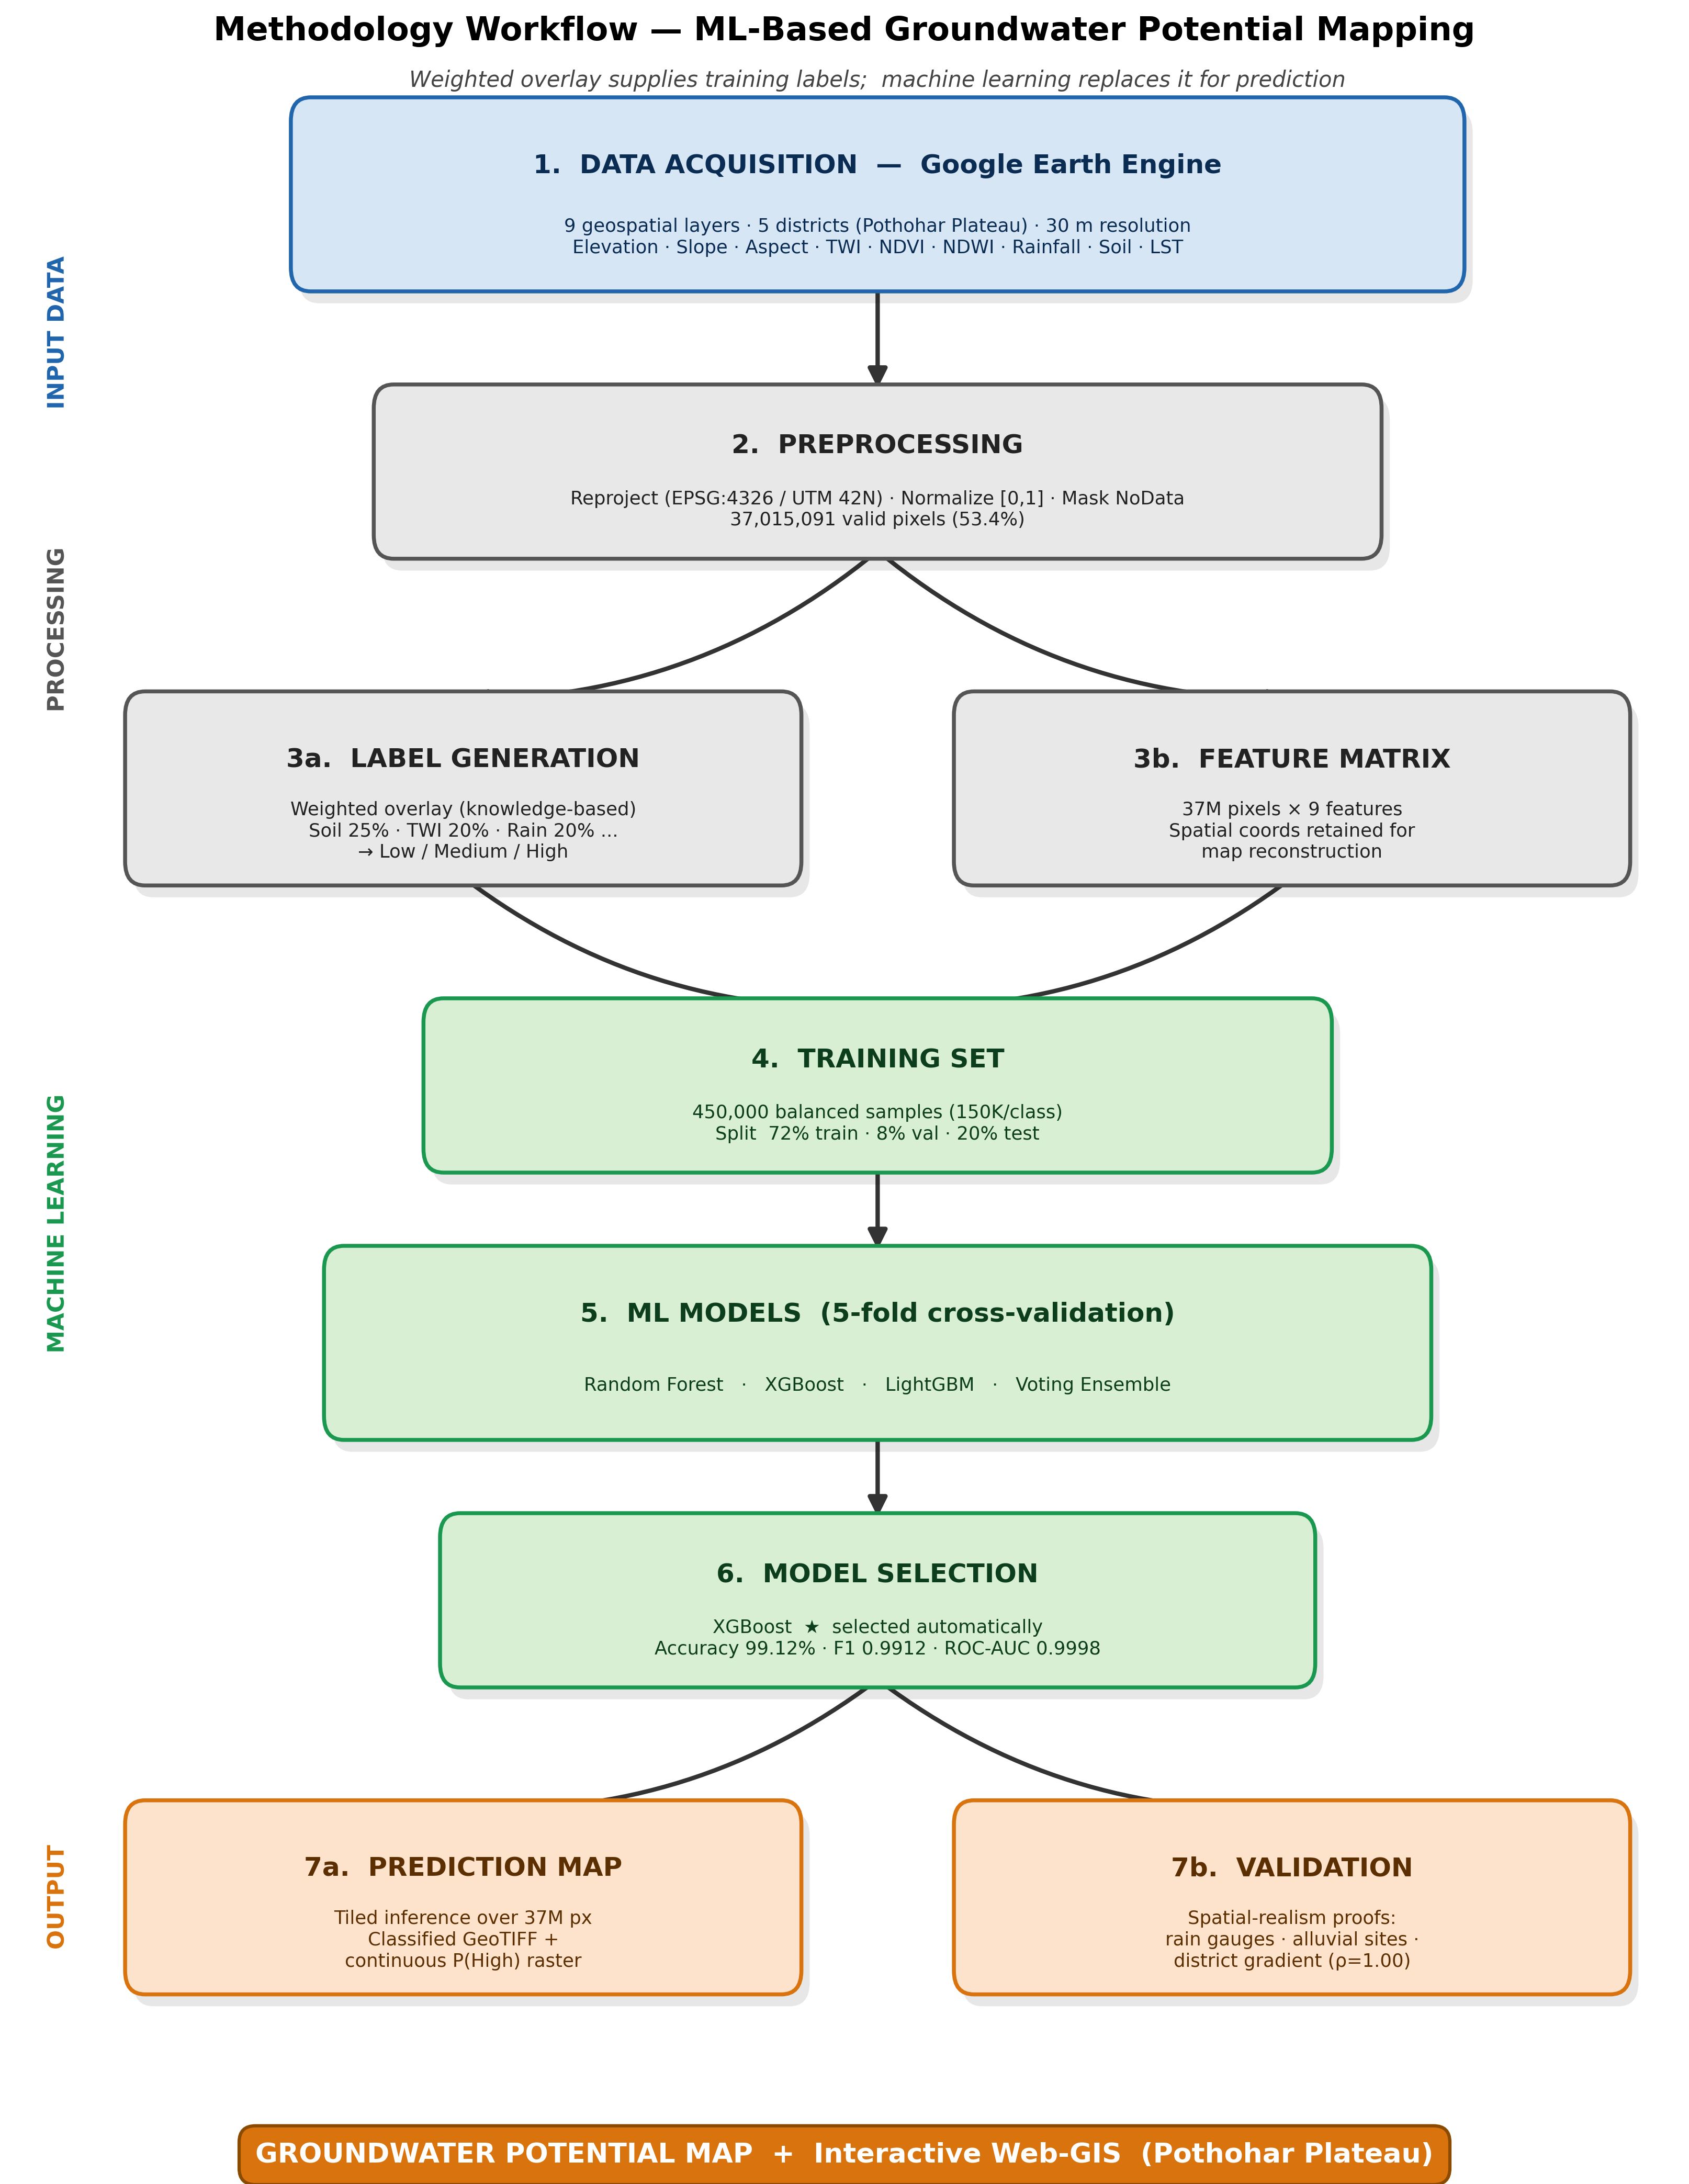
\includegraphics[width=0.92\textwidth]{Fig1_Methodology}
  \caption{Overall methodological workflow, from Google Earth Engine data
           collection through preprocessing, weighted-overlay label generation,
           machine-learning model training, prediction, and spatial-realism
           validation.}
  \label{fig:methodology}
\end{figure}

\section{Data Sources}
\label{sec:data_sources}

Nine features were selected to represent the terrain, climate, vegetation,
moisture, and soil controls on groundwater identified in
Chapter~\ref{ch:literature}. All were obtained through Google Earth Engine,
which provides analysis-ready access to the underlying archives and removes the
need to download and mosaic raw scenes. Table~\ref{tab:data_sources} lists each
feature, its source dataset, and its Pearson correlation with the groundwater
potential label (discussed further in Chapter~\ref{ch:results}).

\begin{table}[H]
\centering
\caption{The nine input features, their source datasets in Google Earth Engine,
         and their Pearson correlation ($r$) with the groundwater potential label.}
\label{tab:data_sources}
\small
\begin{tabular}{clll c}
\toprule
\# & Feature & Source & GEE dataset & $r$ \\
\midrule
1 & Elevation & SRTM            & \texttt{USGS/SRTMGL1\_003}                 & $+0.234$ \\
2 & Slope     & SRTM-derived    & \texttt{ee.Terrain.slope()}                & $+0.051$ \\
3 & Aspect    & SRTM-derived    & \texttt{ee.Terrain.aspect()}               & $+0.060$ \\
4 & TWI       & SRTM + HydroSHEDS & \texttt{WWF/HydroSHEDS/15ACC}            & $+0.185$ \\
5 & NDVI      & Landsat-8       & \texttt{LANDSAT/LC08/C02/T1\_L2}           & $+0.240$ \\
6 & NDWI      & Landsat-8       & \texttt{LANDSAT/LC08/C02/T1\_L2}           & $-0.222$ \\
7 & Rainfall  & CHIRPS          & \texttt{UCSB-CHG/CHIRPS/DAILY}             & $+0.514$ \\
8 & Soil      & SoilGrids       & \texttt{OpenLandMap/SOL/SOL\_TEXTURE}      & $+0.836$ \\
9 & LST       & MODIS           & \texttt{MODIS/061/MOD11A1}                 & $-0.426$ \\
\bottomrule
\end{tabular}
\end{table}

Three of these sources warrant specific mention. Soil texture was taken from
SoilGrids~2.0 \cite{poggio2021soilgrids}, a global digital soil-mapping product
generated with quantile regression forests trained on roughly 240,000 soil
profiles and more than 400 environmental covariates, with cross-validated,
spatially explicit uncertainty. It is the most comprehensive openly available
soil dataset, and---as Chapter~\ref{ch:results} shows---soil texture proved the
single strongest predictor in this study, consistent with its established control
on infiltration and aquifer permeability. The vegetation and water indices (NDVI
and NDWI) were derived from Landsat-8 Collection~2 surface-reflectance imagery
\cite{wulder2019landsat}. The terrain derivatives---elevation, slope, aspect, and
the topographic wetness index---were computed from the 30~m SRTM digital
elevation model; the choice of 30~m resolution is supported by Chang et al.
\cite{chang2019scaleeffects}, who found 30~m DEM derivatives to give the best
model accuracy among the resolutions they tested. The topographic wetness index
itself follows the standard TOPMODEL formulation of Beven and Kirkby
\cite{beven1979topmodel}, combining upslope contributing area (from the
HydroSHEDS flow-accumulation grid) with local slope, and cumulative rainfall was
summed from CHIRPS daily precipitation over the 2015--2023 period.

\section{Data Collection and Export}
\label{sec:collection}

Each feature was assembled in GEE as a single-band image, clipped to the union
of the five FAO/GAUL district polygons, and cast to floating point to avoid
type-mismatch errors when bands of different native types are combined. The nine
bands were stacked and exported as a single multi-band GeoTIFF at 30~m
resolution in geographic coordinates (EPSG:4326). The exported raster spans
$10{,}062 \times 6{,}884$ pixels---about 69.2~million cells---of which
\npixels{} (53.4\%) fall inside the district boundaries and carry valid data;
the remainder are nodata outside the study area. For metric calculations such as
area and distance, the data were reprojected to UTM Zone~42N (EPSG:32642).

\section{Preprocessing}
\label{sec:preprocessing}

Three preprocessing steps prepared the exported stack for analysis, all
implemented in Python with the \texttt{rasterio} library. First, pixels outside
the five district polygons were masked to nodata, fixing the valid-pixel count at
\npixels{}. Second, each band was independently rescaled to the interval
$[0,1]$ by min--max normalization (Equation~\ref{eq:minmax}), so that features
measured in very different units---metres, degrees, millimetres, index values---
contribute on a common scale and no single feature dominates by magnitude alone:

\begin{equation}
  x_{\text{norm}} = \frac{x - x_{\min}}{x_{\max} - x_{\min}}.
  \label{eq:minmax}
\end{equation}

Third, a quality check confirmed that all nine bands contained no missing values
within the valid mask and that every normalized band spanned the full $[0,1]$
range, ruling out constant or degenerate layers. The normalized stack and a
parallel table of pixel row/column indices (used later to reconstruct maps from
tabular predictions) formed the input to all subsequent steps.

\section{Feature Maps}
\label{sec:feature_maps}

Figure~\ref{fig:feature_panel} presents the nine normalized feature layers across
the plateau. Several of the spatial patterns anticipated in
Section~\ref{sec:study_area} are visible: rainfall and vegetation increase toward
the wetter north and northeast, surface temperature is highest over the exposed
southern terrain, and the wetness index picks out the valley floors and
low-lying tracts. These layers are the common input both to the weighted-overlay
labelling described next and to the machine-learning models.

\begin{figure}[H]
  \centering
  \includegraphics[width=\textwidth]{Fig3_Feature_Maps_Panel}
  \caption{The nine normalized geo-environmental input features across the
           \studyarea{}: elevation, slope, aspect, topographic wetness index,
           NDVI, NDWI, rainfall, soil texture, and land surface temperature.}
  \label{fig:feature_panel}
\end{figure}

\section{Label Generation by Weighted Overlay}
\label{sec:labels}

Because field measurements of groundwater are not available across the whole
plateau, reference labels for supervised training were generated using a
knowledge-based weighted overlay---an established approach in GIS-based spatial
mapping, and the same family of method used by the reference study
\cite{waqas2022chakwal} and validated as a labelling strategy by Roy and Saha
\cite{roy2019knowledgedriven} and others \cite{arulbalaji2019gisahp,pande2021ahpmif}.
Each normalized feature $f_i$ was assigned a weight $w_i$ reflecting its
hydrogeological influence on groundwater potential, and the weights were combined
into a single composite score $S$ for every pixel:

\begin{equation}
  S = \sum_{i=1}^{9} w_i \, f_i^{*},
  \label{eq:overlay}
\end{equation}

where $f_i^{*} = f_i$ for features that promote groundwater and
$f_i^{*} = 1 - f_i$ for features that suppress it. Features inversely related to
potential---slope, elevation, and land surface temperature---were inverted in
this way before weighting, so that, for instance, gentler slopes and cooler
(less evaporative) surfaces raise the score. The weights, listed in
Table~\ref{tab:weights}, give the largest influence to soil texture, the wetness
index, and rainfall, in line with both the hydrogeology of the area and the
correlations in Table~\ref{tab:data_sources}.

\begin{table}[H]
\centering
\caption{Feature weights and direction of influence used in the weighted-overlay
         label generation.}
\label{tab:weights}
\begin{tabular}{lcc}
\toprule
Feature & Weight (\%) & Direction \\
\midrule
Soil texture & 25 & Direct ($+$) \\
TWI          & 20 & Direct ($+$) \\
Rainfall     & 20 & Direct ($+$) \\
NDVI         & 10 & Direct ($+$) \\
Slope        & 10 & Inverse ($-$) \\
NDWI         &  5 & Direct ($+$) \\
Elevation    &  5 & Inverse ($-$) \\
LST          &  3 & Inverse ($-$) \\
Aspect       &  2 & Direct ($+$) \\
\midrule
\textbf{Total} & \textbf{100} & \\
\bottomrule
\end{tabular}
\end{table}

The continuous score was then divided into three ordinal classes using fixed
percentile thresholds: the lowest 40\% of scores were labelled \emph{Low}
potential (class~0), the 40th--80th percentile \emph{Medium} (class~1), and the
top 20\% \emph{High} (class~2). This 40/40/20 split reflects the expectation that
high-potential ground is the minority of a semi-arid plateau, and it fixes the
overall class balance of the reference map. The resulting label map is shown in
Figure~\ref{fig:label_map}.

\begin{figure}[H]
  \centering
  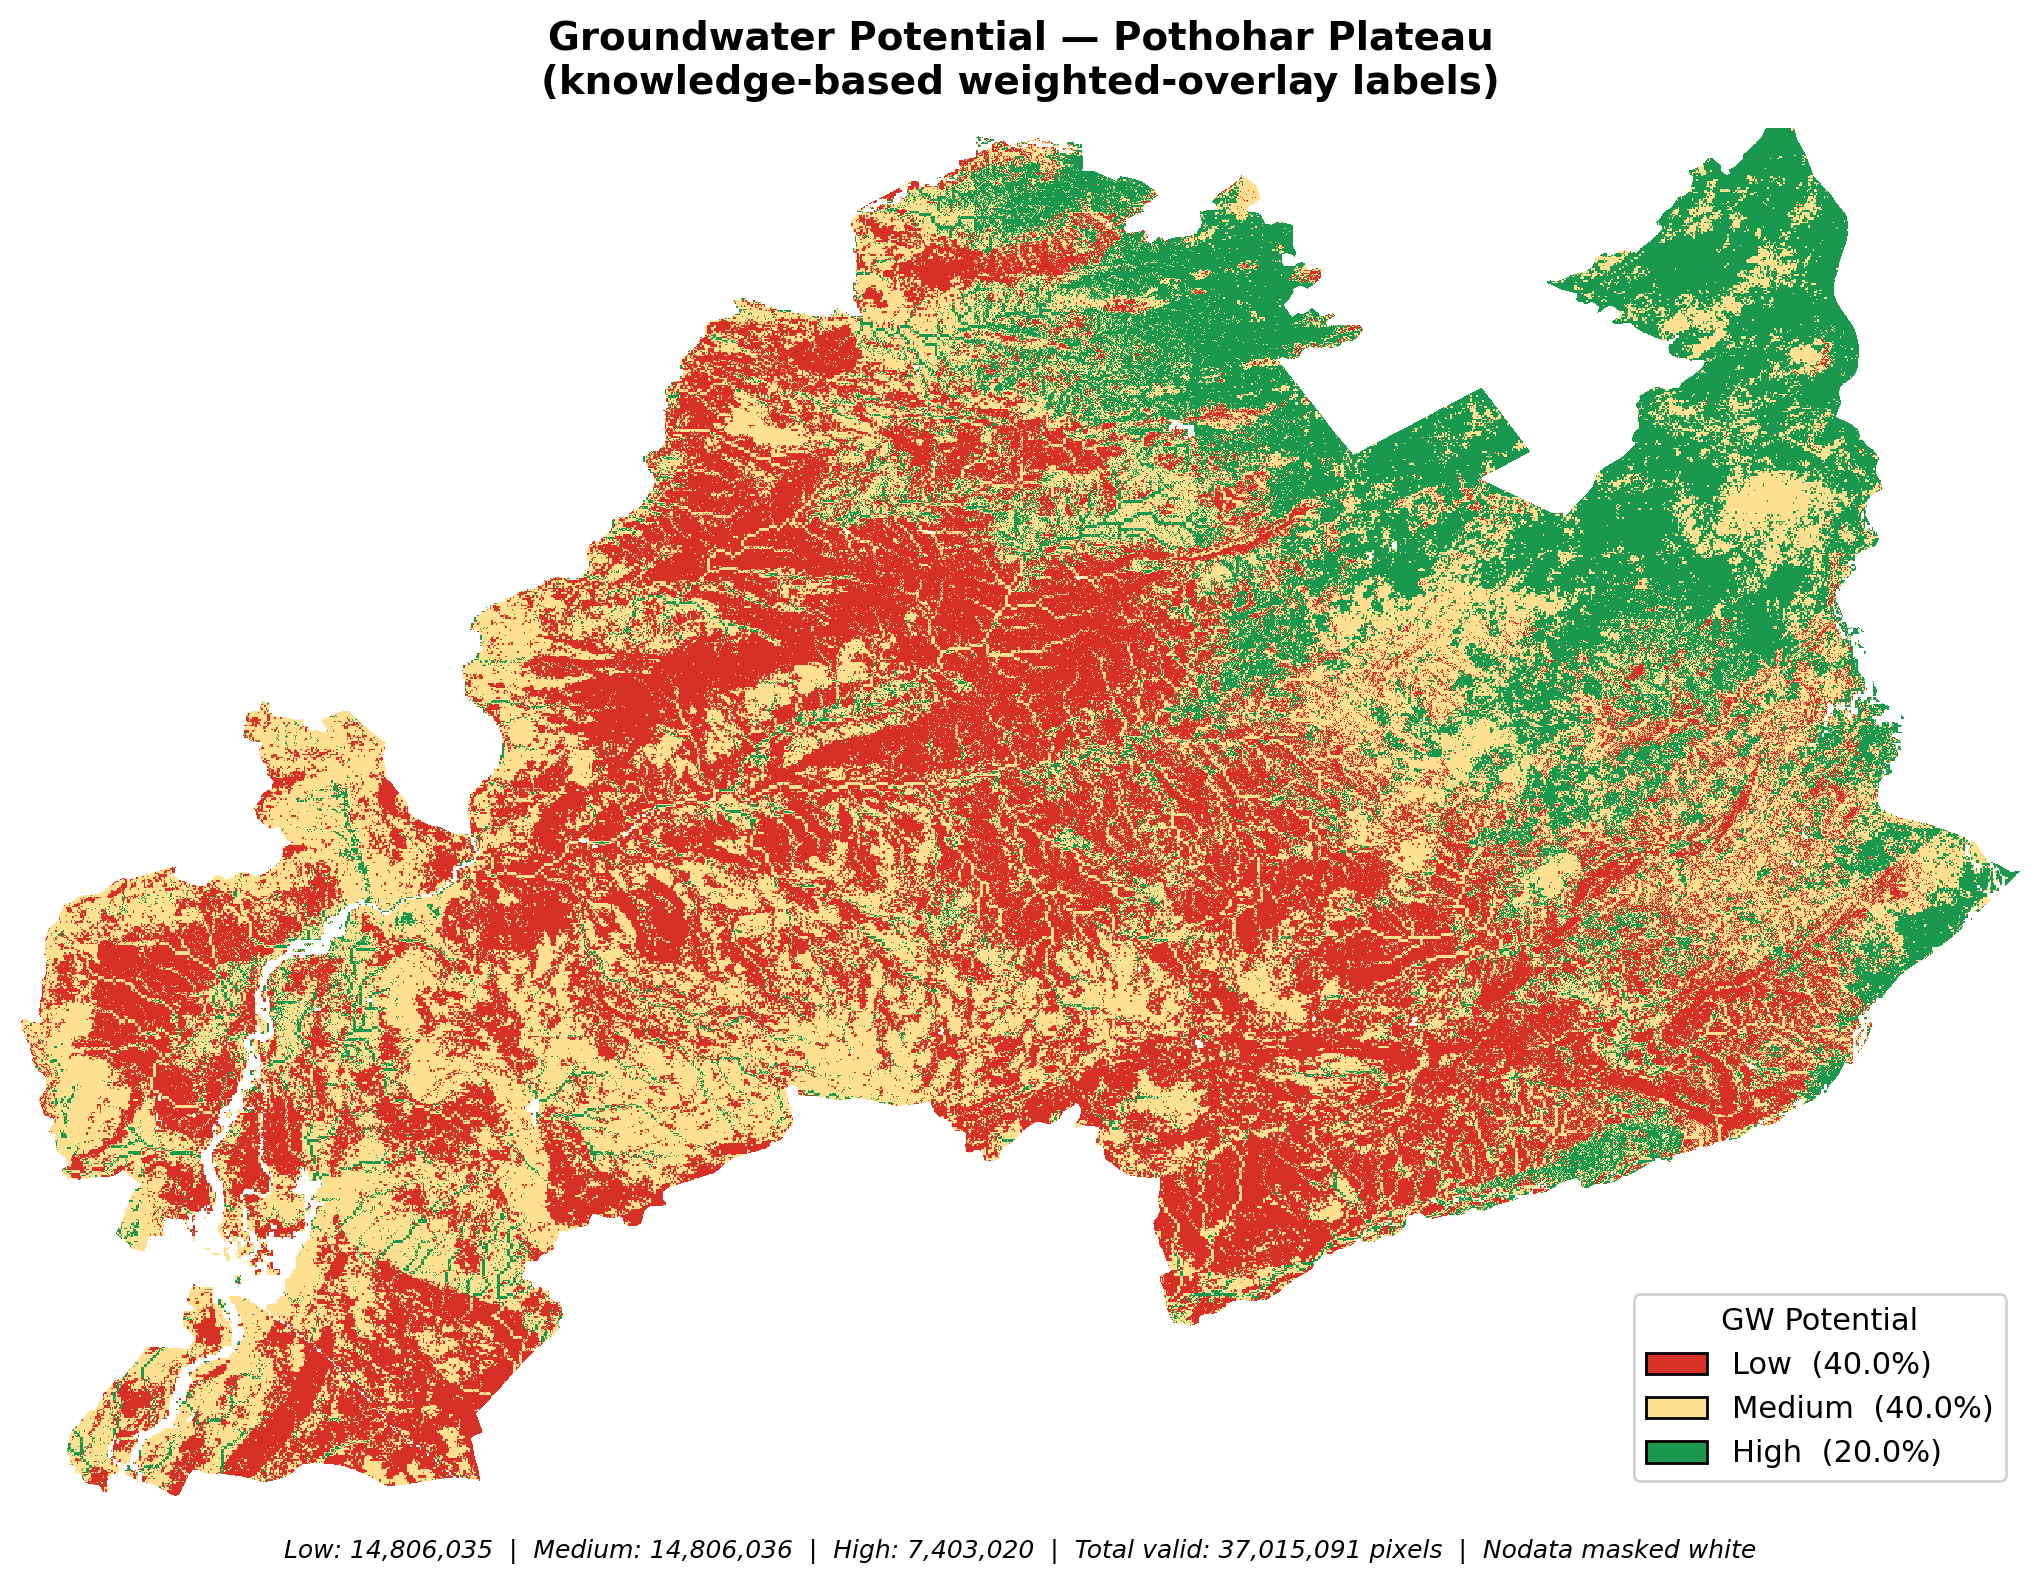
\includegraphics[width=0.85\textwidth]{gw_potential_label_map}
  \caption{Groundwater potential reference labels generated by the
           weighted-overlay model: Low (40\%), Medium (40\%), and High (20\%)
           potential zones across the \studyarea{}.}
  \label{fig:label_map}
\end{figure}

It is worth restating plainly what these labels are and are not. They encode
hydrogeological knowledge applied to the satellite features, not direct
observations of groundwater. A model trained on them therefore learns to
reproduce that knowledge-based product, and its internal accuracy measures
fidelity to the overlay rather than to ground truth. This is an accepted
limitation of GWPM in data-scarce regions; the response adopted here is not to
pretend otherwise but to validate the final map against independent evidence, as
described in Section~\ref{sec:validation_design} and Chapter~\ref{ch:results}.

\section{Training Dataset Construction}
\label{sec:training_data}

Training every model on all \npixels{} labelled pixels would be both
computationally wasteful and statistically skewed by the fixed 40/40/20 class
proportions. Instead, a balanced sample of 450,000 pixels was drawn---150,000
from each of the three classes---by stratified random sampling. Balancing the
classes prevents the models from favouring the majority classes and makes
metrics such as macro $F_1$ directly interpretable. The sample was partitioned
into 72\% training, 8\% validation, and 20\% test subsets, leaving 90,000 pixels
held out for final evaluation. The decision to fix and report this split
explicitly follows Nguyen et al. \cite{nguyen2021datasplitting}, who showed that
the partitioning scheme materially affects reported performance and should not be
left implicit.

\section{Machine-Learning Models}
\label{sec:ml_models}

Four classifiers were trained on the same data so that their performance could be
compared directly. They were chosen to span the two dominant tree-ensemble
strategies---bagging and boosting---and their combination:

\begin{itemize}
  \item \textbf{Random Forest (RF).} An ensemble of 300 decision trees grown on
        bootstrapped samples with Gini-impurity splits and a $\sqrt{9}$ feature
        subsample at each node \cite{liaw2007randomforest,tyralis2019randomforests}.
  \item \textbf{XGBoost.} Regularized gradient-boosted trees
        \cite{chen2016xgboost}, with learning rate 0.1, maximum depth 6, 300
        estimators, and 0.8 row/column subsampling.
  \item \textbf{LightGBM.} Histogram-based, leaf-wise gradient boosting
        \cite{ke2017lightgbm}, with 500 estimators, learning rate 0.05, and a
        minimum of 30 samples per leaf.
  \item \textbf{Voting Ensemble.} A soft-voting combination of the three models
        above with equal weights, averaging their predicted class probabilities.
\end{itemize}

All models were implemented in Python using \texttt{scikit-learn},
\texttt{xgboost}, and \texttt{lightgbm}. The comparison is deliberately aligned
with prior susceptibility-mapping work---most directly Sahin
\cite{sahin2020ensembletree}, who compared the same boosting and bagging
families---so that the model ranking obtained here can be read against an
external benchmark.

\section{Evaluation Metrics}
\label{sec:metrics}

Model performance was assessed on the 90,000-pixel test set using several
complementary measures rather than accuracy alone, since accuracy can be
misleading even on balanced data. Overall accuracy is reported alongside the
macro-averaged $F_1$-score, which weights all three classes equally; Cohen's
$\kappa$, which corrects agreement for chance; and the one-vs-rest ROC-AUC, which
summarizes class separability across decision thresholds. Per-class precision,
recall, and $F_1$ are also reported. The use of agreement- and
separability-based measures in addition to raw accuracy follows the
recommendation of Chicco and Jurman \cite{chicco2020mcc}. To confirm that the
results were not an artefact of a single partition, each model was additionally
evaluated under five-fold cross-validation on the training set.

\section{Prediction Map Generation}
\label{sec:prediction}

The best-performing model was then applied to all \npixels{} valid pixels to
produce the full-resolution groundwater potential map. Because holding the entire
feature stack in memory at once is impractical, prediction was carried out over
the raster in $2048 \times 2048$ pixel tiles, with each tile's pixels classified
in turn and written back to the output grid---twenty tiles in total, completing in
roughly twenty minutes. Two outputs were produced: a classified GeoTIFF assigning
each pixel to Low, Medium, or High potential, and a continuous raster giving the
model's predicted probability of the High class, which preserves the gradational
information lost in the hard classification and is used in the validation that
follows.

\section{Validation Design}
\label{sec:validation_design}

The central difficulty in validating this map is the one already noted: the
training labels are themselves model-derived, so a high agreement between the
prediction and the labels (reported in Chapter~\ref{ch:results}) confirms only
that the learning succeeded, not that the map is hydrogeologically correct. A
conventional well-by-well accuracy assessment was attempted but proved
uninformative, because the publicly available monitoring wells for the region are
not classified as productive or dry---they exist across both favourable and
unfavourable ground---and many fell on nodata pixels at the district margins.

The approach taken instead is what is termed here a \emph{spatial-realism
validation}: rather than asking whether the map matches a noisy point-by-point
ground truth, it asks whether the map's spatial structure agrees with independent
lines of hydrogeological evidence. Four such checks were designed:

\begin{enumerate}
  \item \textbf{Known productive sites.} Published groundwater sites in the
        Rawalpindi alluvial basin---ground that is known to be productive---were
        overlaid on the map, and the predicted class and High-probability at each
        were examined. A credible map should place these in the Medium or High
        classes.
  \item \textbf{Recharge-zone discrimination.} The independent network of
        rain-gauge stations compiled by Khan et al. \cite{khan2023rainfallrunoff}
        across the Pothohar basins was partitioned by hydrogeological setting into
        alluvial and non-alluvial groups, and the predicted High-probability was
        compared between groups using the Mann--Whitney $U$ test. Alluvial
        stations should show significantly higher predicted potential.
  \item \textbf{Cross-study consistency.} The predicted proportion of High
        potential was compared against the suitability proportions reported by an
        independent AHP study of the same region \cite{hafeez2025rwh}, to check
        that the overall magnitude is consistent with prior regional work.
  \item \textbf{District-scale gradient.} The fraction of each district classified
        as High potential was ranked and tested against the expected
        hydrogeological ordering (wetter, alluvial north versus drier, hard-rock
        south) using the Spearman rank correlation.
\end{enumerate}

Together these checks assess whether the map is right for the right reasons,
using evidence that played no part in its construction. Their results are
reported in Section~\ref{sec:validation_results}, and their interpretation, along
with the limitations of the approach, is taken up in
Chapter~\ref{ch:discussion}.

% ============================================================
%  Chapter 4 — Results
% ============================================================
\chapter{Results}
\label{ch:results}

This chapter reports the outcomes of the analysis in the order the methodology
introduced them: the exploratory structure of the feature data, the comparative
performance of the four classifiers, the factors the best model relied on, the
resulting groundwater potential map, and finally the spatial-realism validation
that tests the map against independent evidence.

\section{Exploratory Data Analysis}
\label{sec:eda}

Before any model was trained, the relationship between each feature and the
groundwater potential label was examined across all \npixels{} valid pixels. The
nine features contained no missing values within the study-area mask and each
spanned the full normalized range, so no pixels were lost to incomplete data.

The Pearson correlations (Figure~\ref{fig:correlation}) are informative in their
own right. Soil texture stands out, correlating with the potential label at
$r = 0.836$---far stronger than any other feature---followed by cumulative
rainfall at $r = 0.514$. Land surface temperature is the strongest of the
negatively associated features ($r = -0.426$), consistent with its role as a
proxy for evaporative loss. NDVI ($+0.240$), elevation ($+0.234$), NDWI
($-0.222$), and TWI ($+0.185$) form a middle group, while aspect ($+0.060$) and
slope ($+0.051$) are effectively uncorrelated. The negligible slope correlation
is itself a regional finding rather than a defect: across a comparatively
subdued plateau, slope simply does not discriminate groundwater zones the way it
would in mountainous terrain.

\begin{figure}[H]
  \centering
  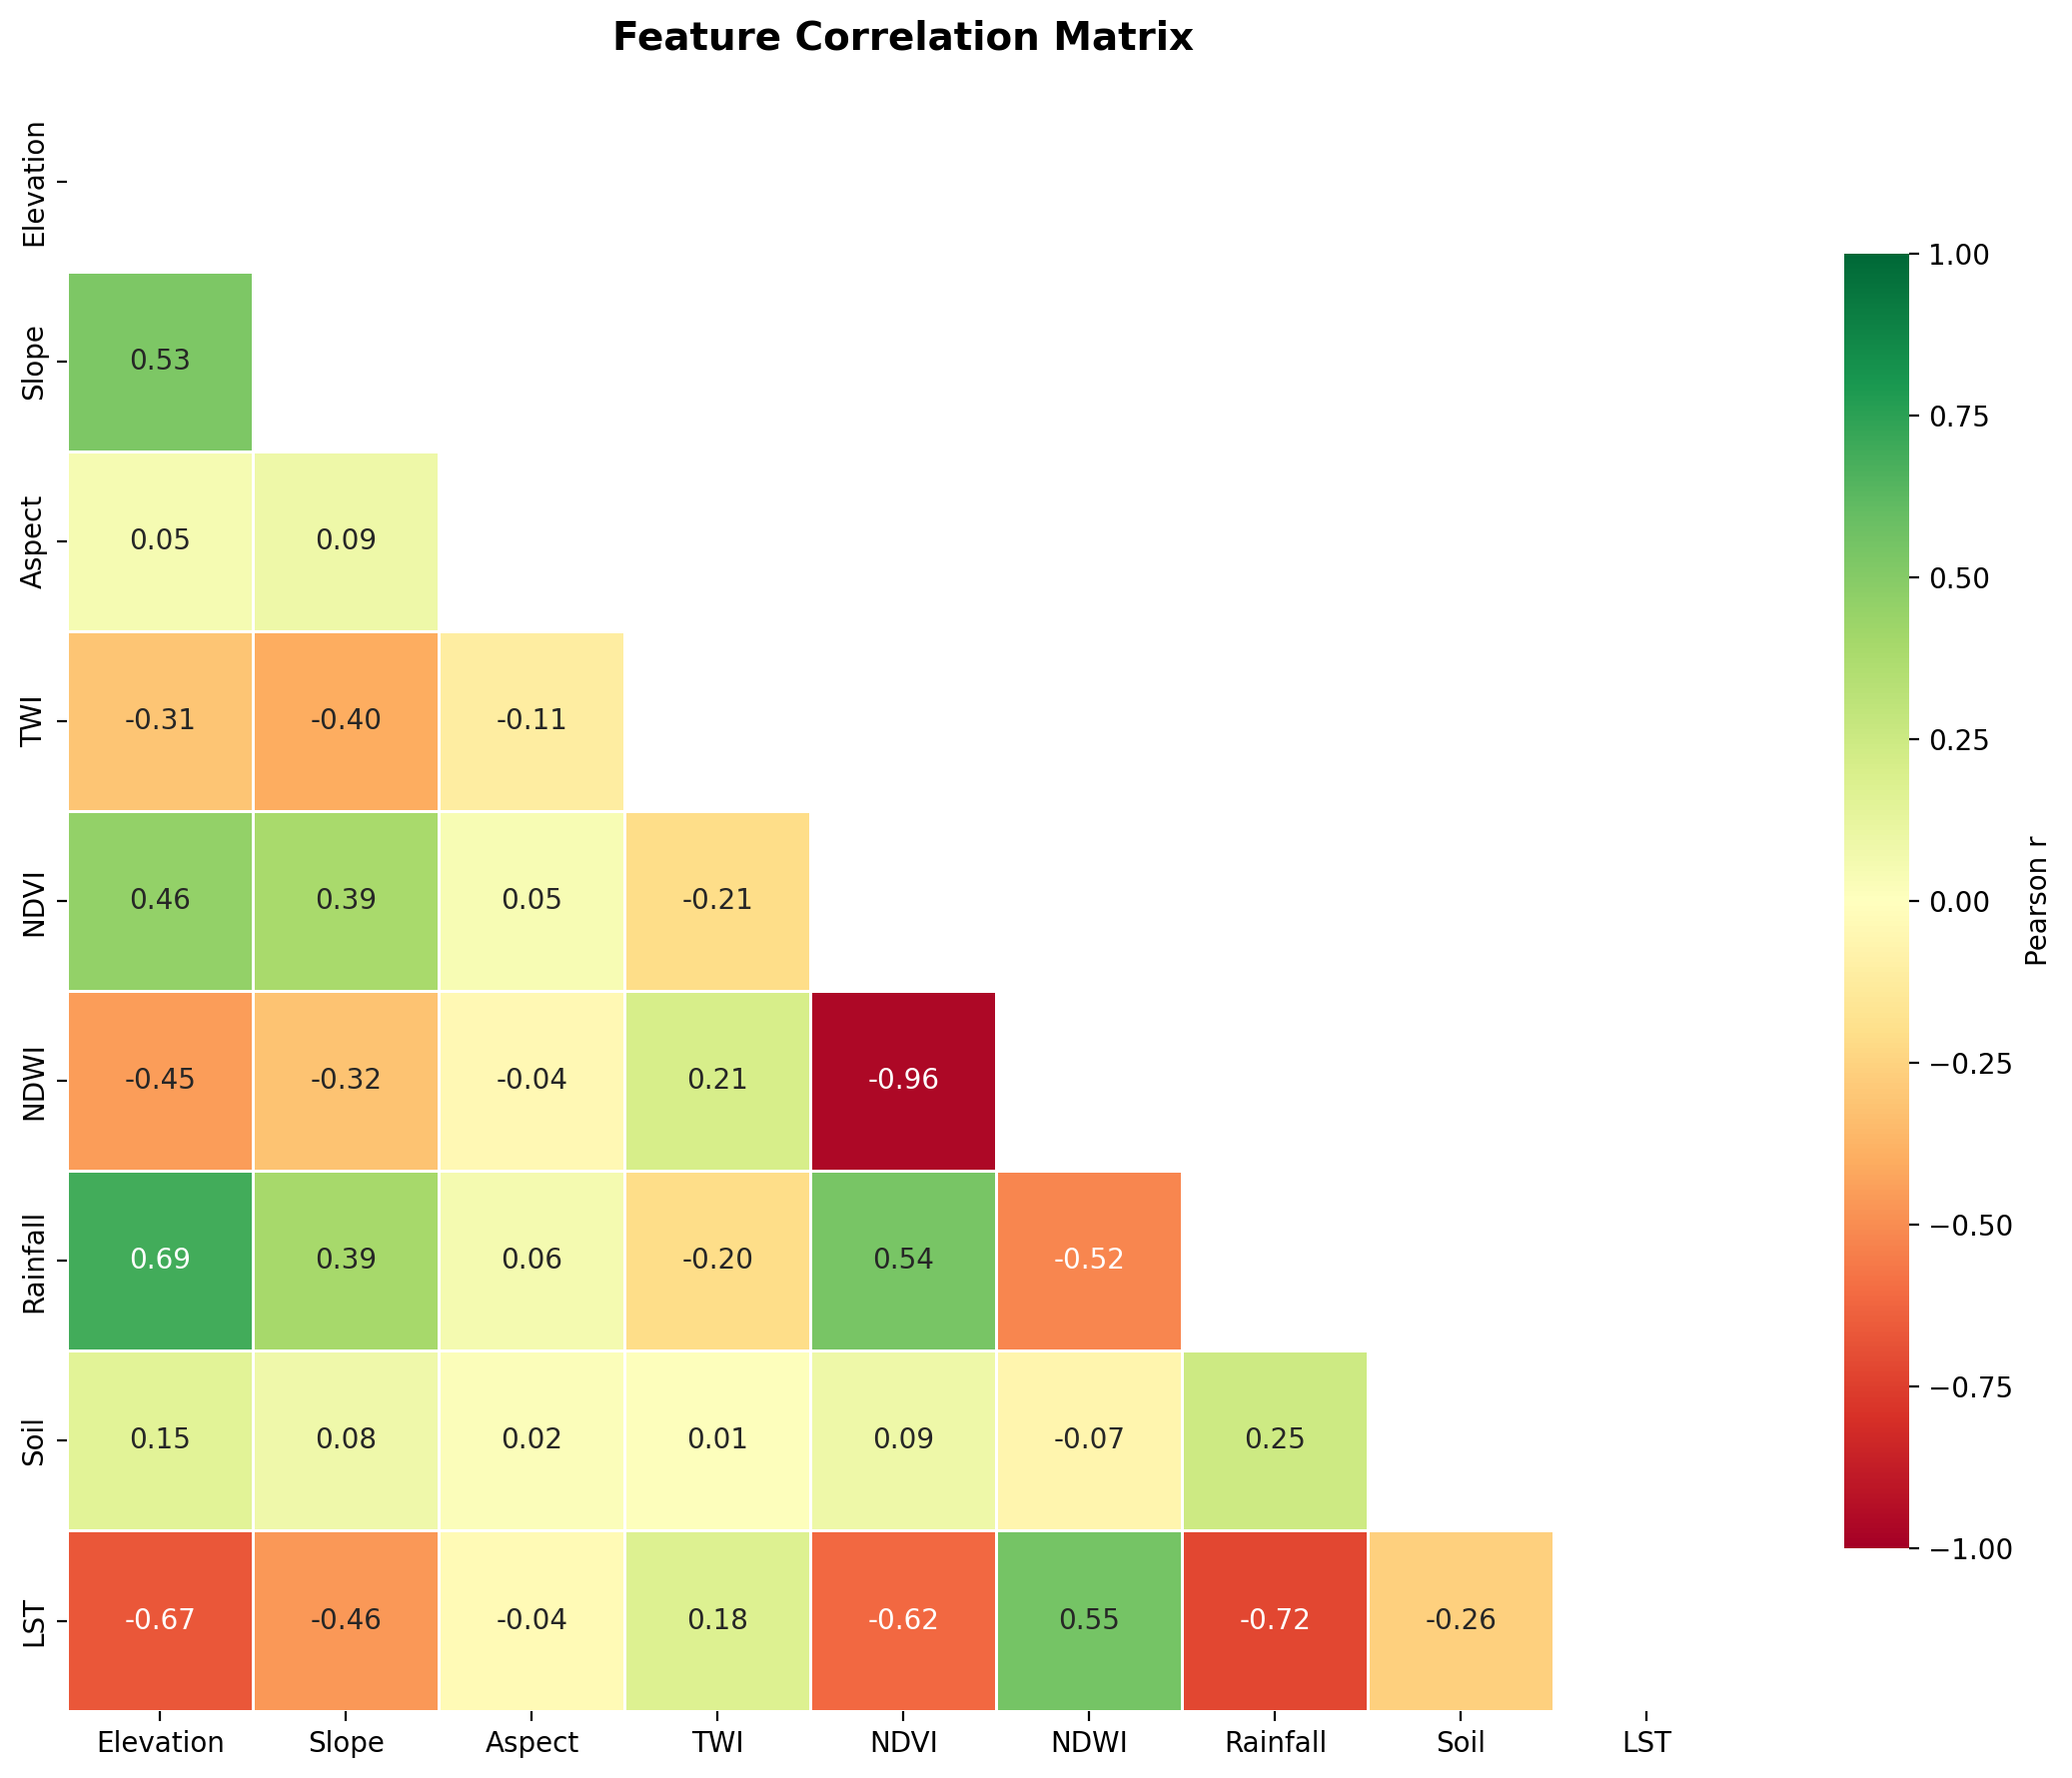
\includegraphics[width=0.8\textwidth]{correlation_matrix}
  \caption{Pearson correlation matrix of the nine input features and the
           groundwater potential label. Soil texture ($r=0.836$) and rainfall
           ($r=0.514$) are the dominant positively correlated predictors.}
  \label{fig:correlation}
\end{figure}

The dominance of soil and rainfall is consistent with the hydrogeology discussed
in Chapter~\ref{ch:methodology} and with the wider literature: permeability
controls whether water infiltrates, and rainfall supplies the water to begin
with. It also echoes Khan et al. \cite{khan2023rainfallrunoff}, who found
rainfall to be the principal driver of the hydrological response in these same
basins. Figure~\ref{fig:feature_target} summarizes the per-feature association
with the label in ranked form.

\begin{figure}[H]
  \centering
  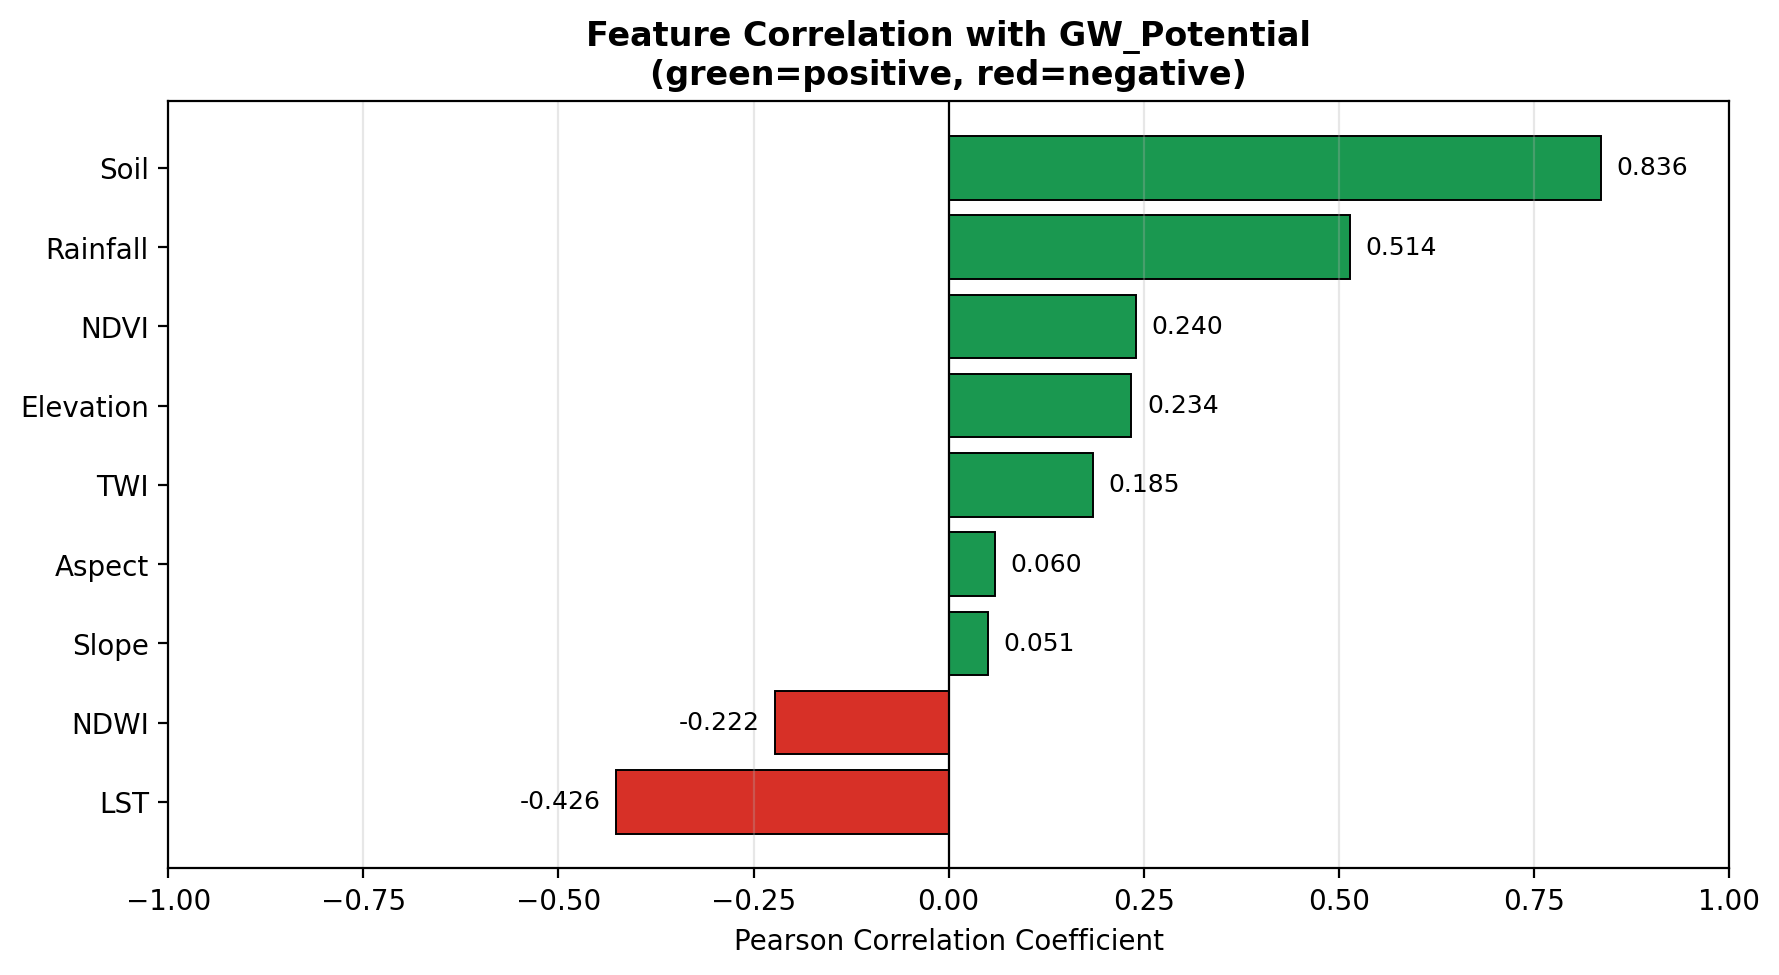
\includegraphics[width=0.75\textwidth]{feature_target_correlation}
  \caption{Features ranked by absolute correlation with the groundwater potential
           label, showing the clear lead of soil texture and rainfall.}
  \label{fig:feature_target}
\end{figure}

By construction, the weighted-overlay labelling produced a class distribution of
40\% Low, 40\% Medium, and 20\% High (Figure~\ref{fig:class_dist}). The balanced
training sample drawn from these labels removed this imbalance for model fitting,
as described in Section~\ref{sec:training_data}.

\begin{figure}[H]
  \centering
  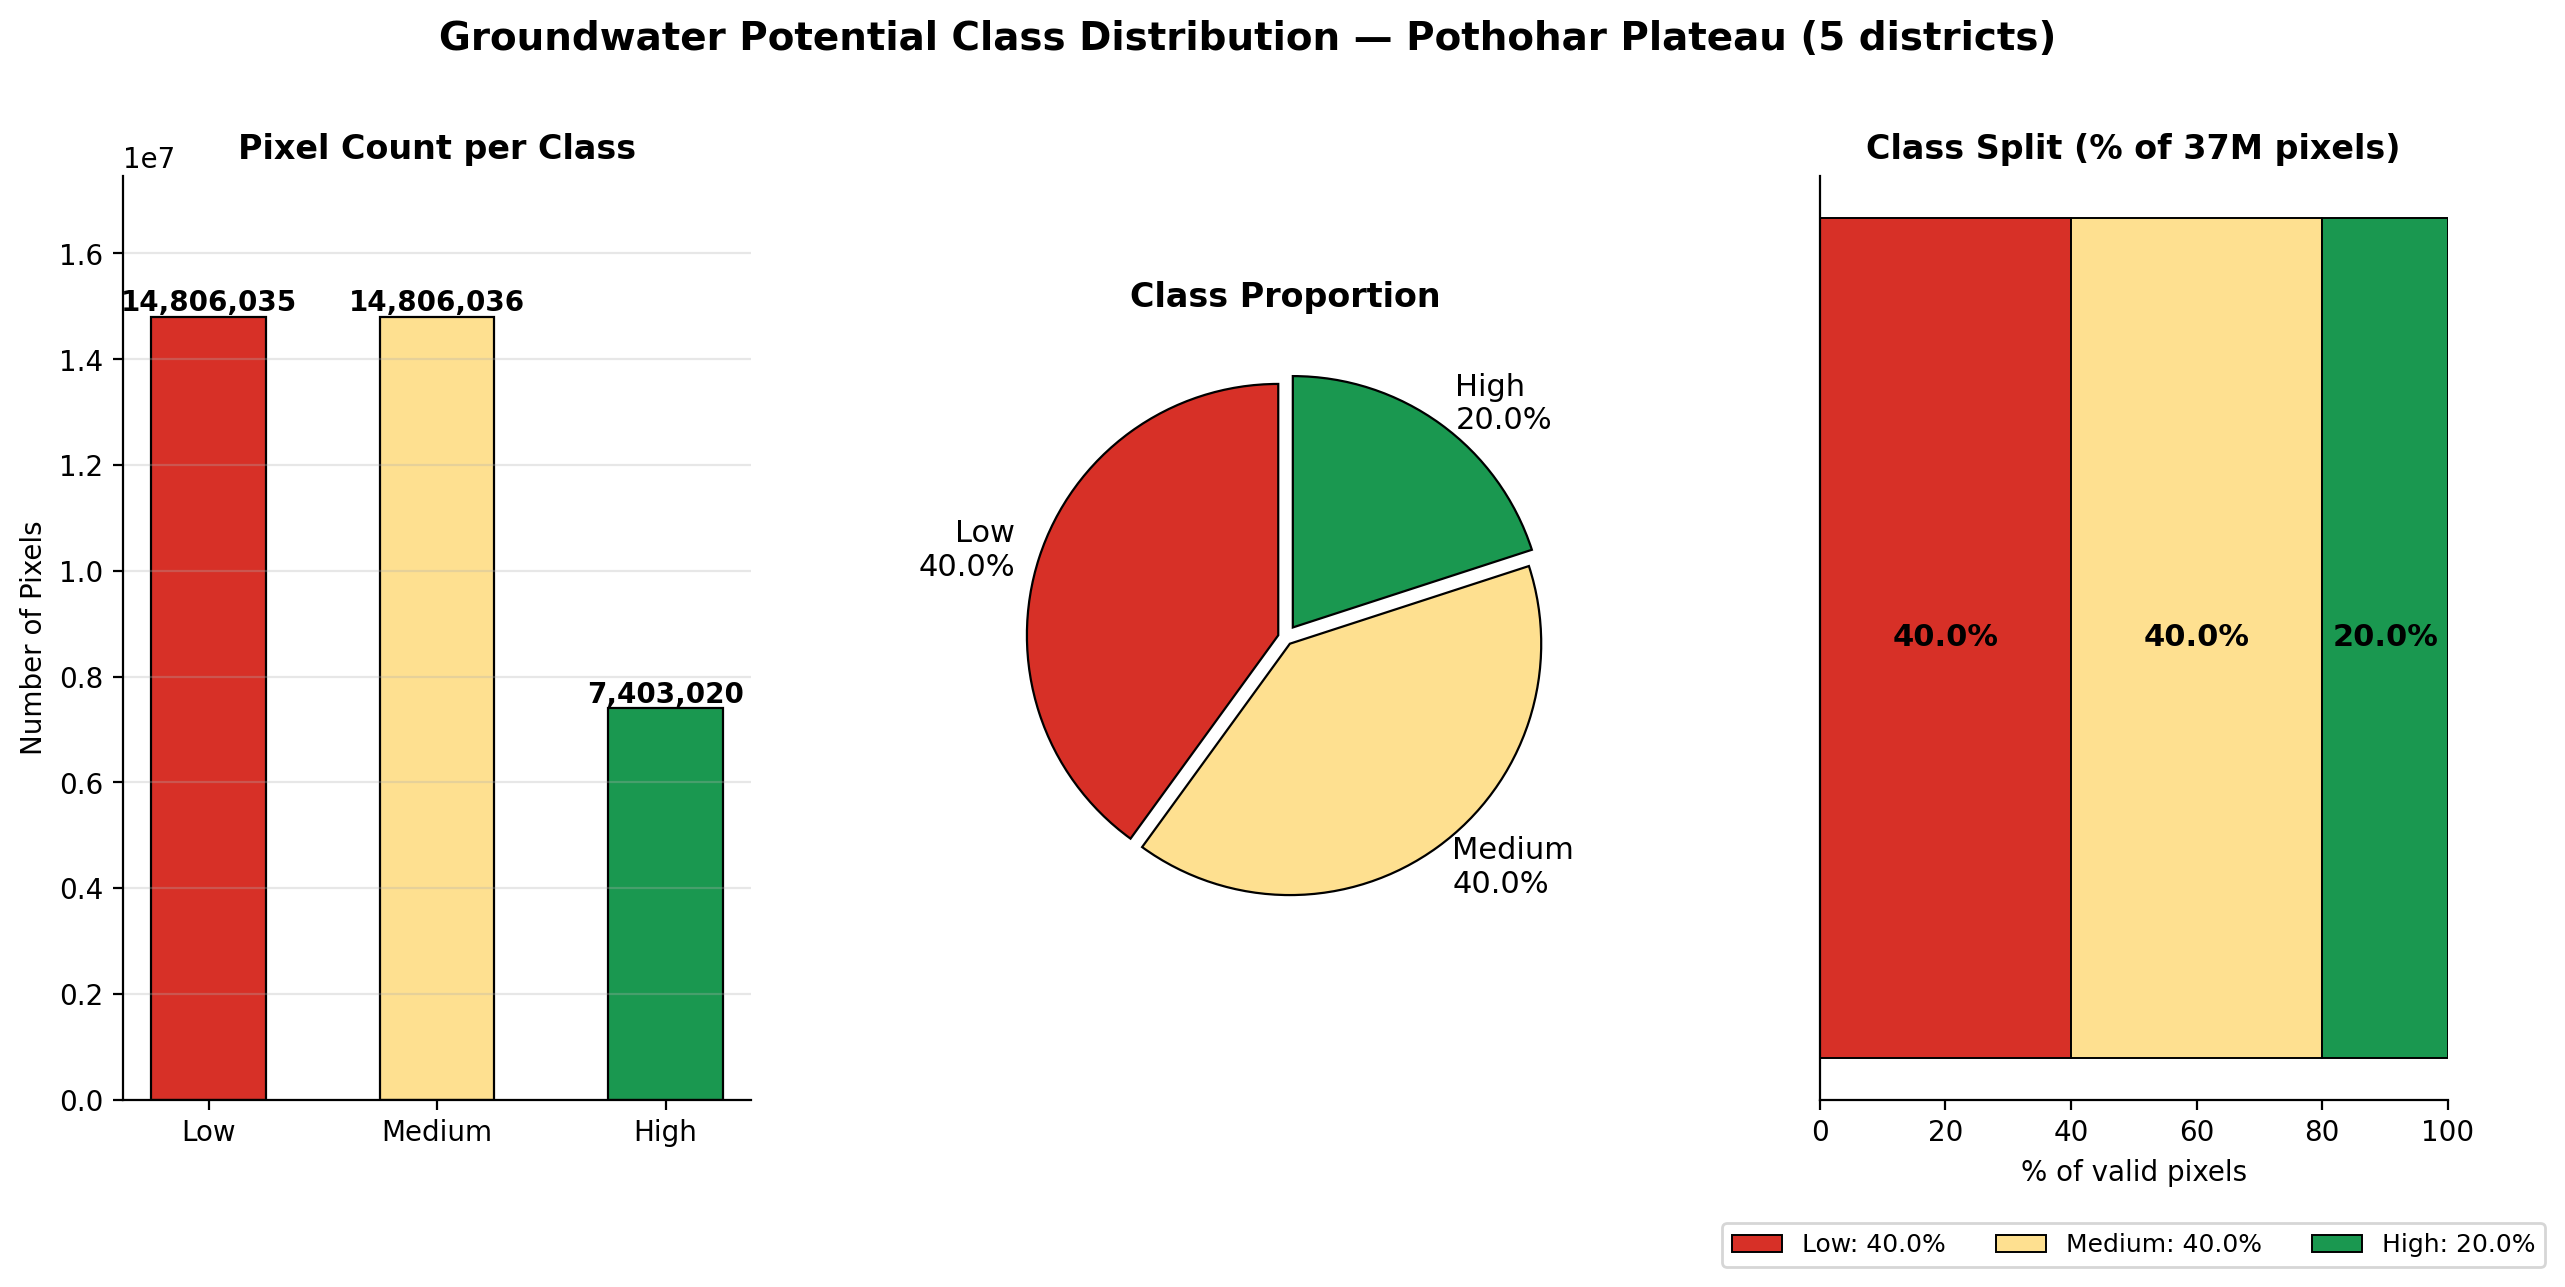
\includegraphics[width=0.7\textwidth]{class_distribution_pub}
  \caption{Distribution of the three groundwater potential classes in the
           weighted-overlay reference labels across the full plateau.}
  \label{fig:class_dist}
\end{figure}

\section{Model Performance}
\label{sec:model_performance}

All four classifiers were trained on the 360,000-pixel training portion and
evaluated on the held-out 90,000-pixel test set.
Table~\ref{tab:model_results} reports the headline metrics.

\begin{table}[H]
\centering
\caption{Performance of the four classifiers on the 90,000-pixel test set. Best
         value in each column in bold.}
\label{tab:model_results}
\begin{tabular}{lcccc}
\toprule
Model & Accuracy (\%) & Macro $F_1$ & Cohen's $\kappa$ & ROC-AUC \\
\midrule
Random Forest      & 98.32 & 0.9832 & 0.9749 & 0.9995 \\
\textbf{XGBoost}   & \textbf{99.12} & \textbf{0.9912} & \textbf{0.9868} & \textbf{0.9998} \\
LightGBM           & 99.11 & 0.9911 & 0.9867 & 0.9998 \\
Voting Ensemble    & 99.09 & 0.9909 & 0.9863 & 0.9998 \\
\bottomrule
\end{tabular}
\end{table}

XGBoost gave the best results on every metric, reaching 99.12\% accuracy, a macro
$F_1$ of 0.9912, Cohen's $\kappa$ of 0.9868, and a one-vs-rest ROC-AUC of 0.9998,
and it was selected as the model for full-plateau prediction. The margins between
the top three models are slim---LightGBM trails by barely a hundredth of a
percentage point, and the voting ensemble sits just behind both---while random
forest is a clear, if still strong, step below at 98.32\%. This ordering, with
XGBoost ahead of random forest and gradient boosting clustered at the top, mirrors
the ranking Sahin \cite{sahin2020ensembletree} reported for the same model
families in landslide susceptibility mapping, which lends some external
credibility to the comparison even though the absolute numbers here are higher.
Figure~\ref{fig:model_comparison} shows the comparison visually.

\begin{figure}[H]
  \centering
  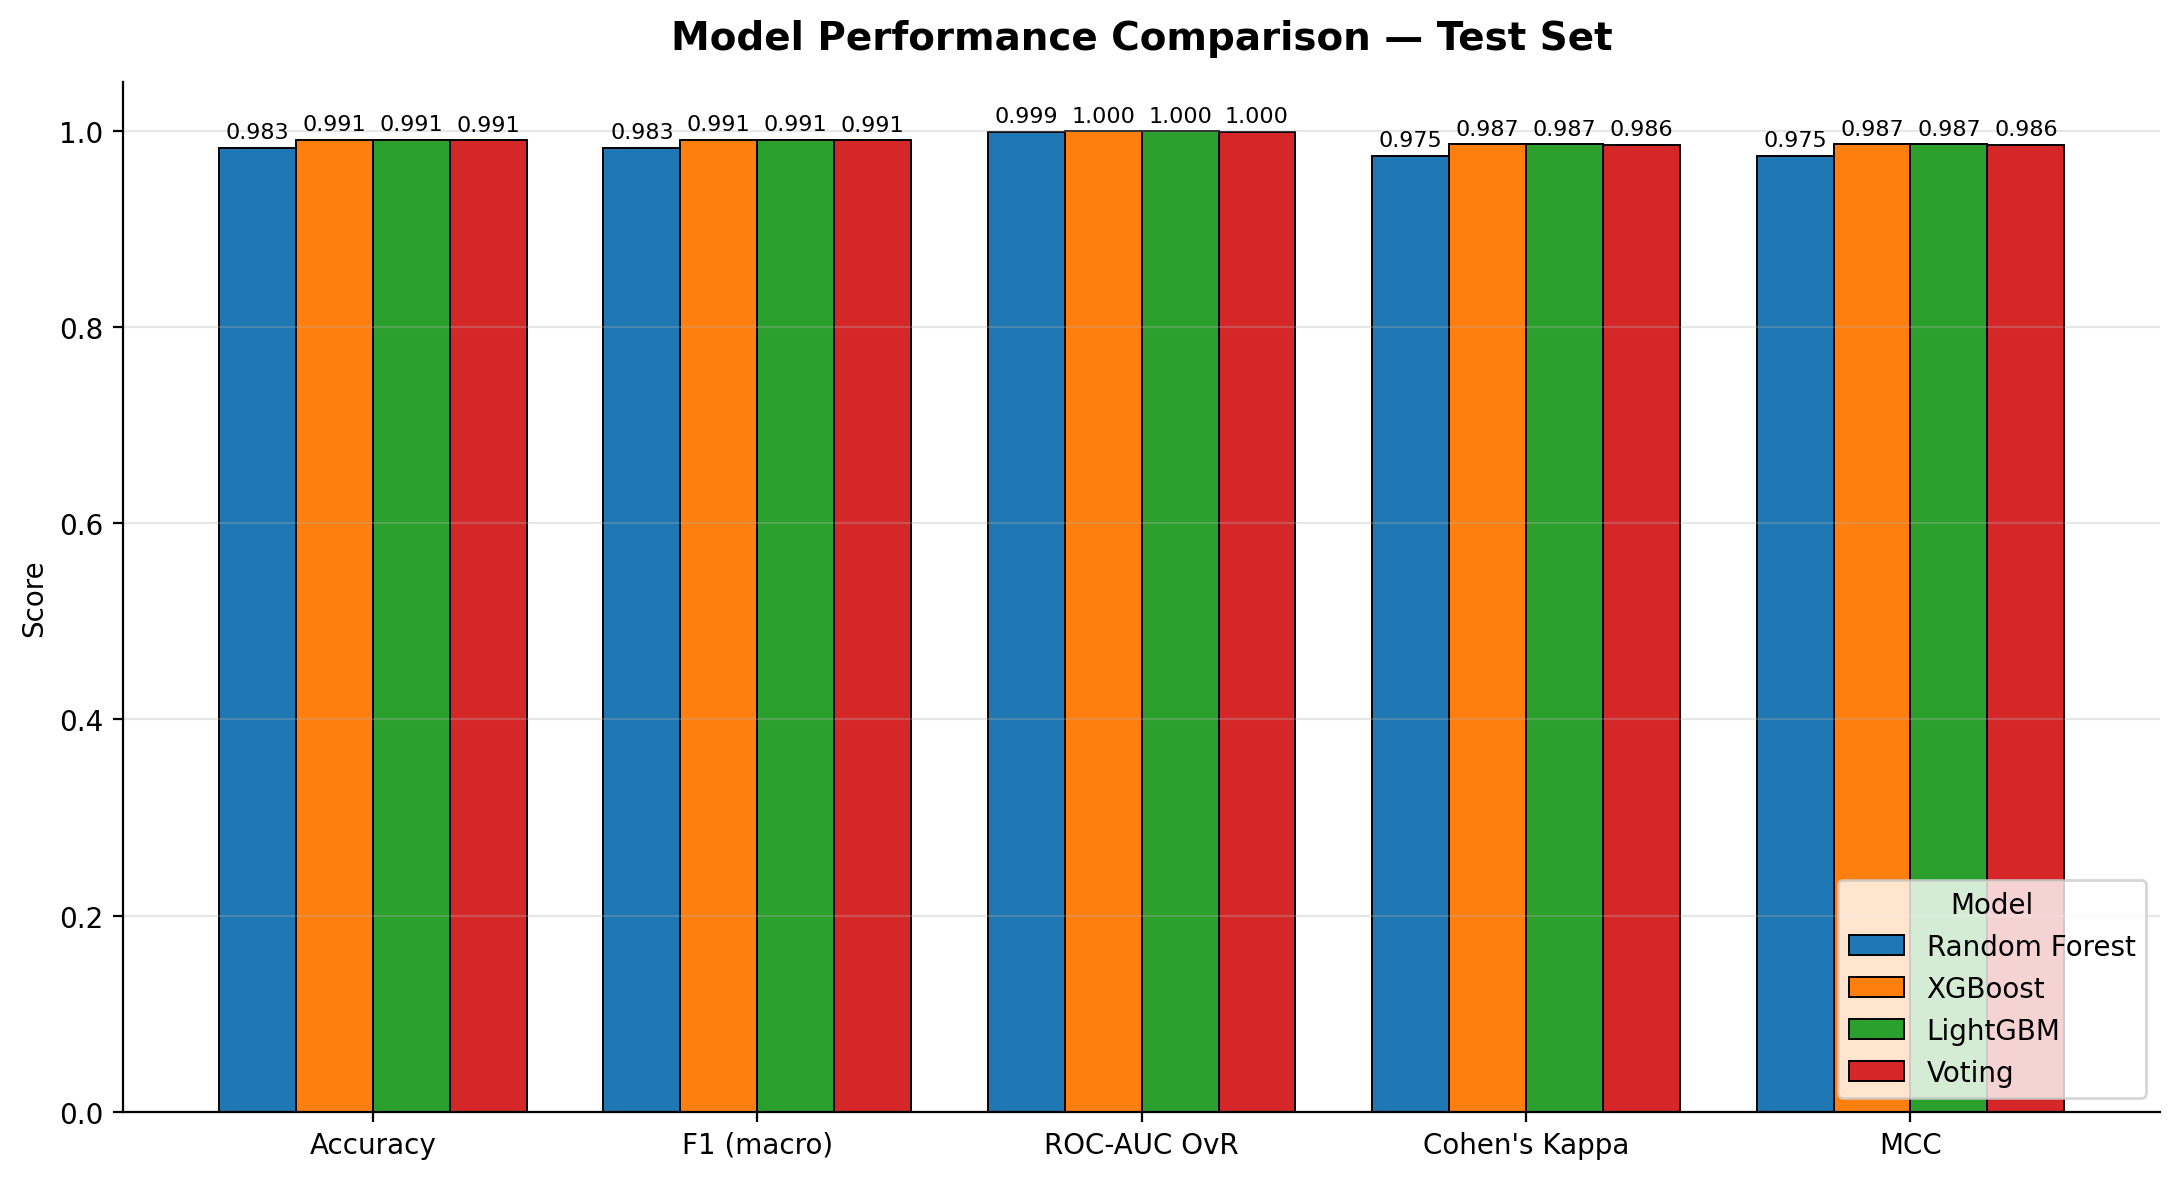
\includegraphics[width=0.85\textwidth]{model_comparison}
  \caption{Comparison of the four classifiers across accuracy, macro $F_1$,
           Cohen's $\kappa$, and ROC-AUC on the test set.}
  \label{fig:model_comparison}
\end{figure}

The absolute accuracies---near 99\%---are far above the 0.73--0.86 AUC range
typical of knowledge-driven AHP and frequency-ratio GWPM studies
\cite{das2018pravara,pande2021ahpmif}. This gap should be read carefully rather
than celebrated uncritically: it reflects in large part the fact that the models
are learning to reproduce a deterministic weighted overlay built from the same
features, a point developed in Section~\ref{sec:agreement} and again in
Chapter~\ref{ch:discussion}. What the metrics establish is that the learning
problem was solved cleanly; whether the resulting map is hydrogeologically
trustworthy is a separate question, addressed by the validation in
Section~\ref{sec:validation_results}.

\subsection{Per-Class Performance}
\label{sec:per_class}

Because a high overall accuracy can still hide weakness on a minority class, the
per-class behaviour of XGBoost was examined (Table~\ref{tab:per_class}). All
three classes are predicted with precision and recall above 98\%. The High class,
the one of greatest practical interest, is recovered with the highest recall of
the three (99.61\%), meaning the model rarely misses genuinely high-potential
ground in the test set; the slightly lower precision and recall on the Medium
class reflect the expected difficulty of the middle category, whose boundaries
with Low and High are the least sharp.

\begin{table}[H]
\centering
\caption{Per-class precision, recall, and $F_1$ for the XGBoost model on the
         test set.}
\label{tab:per_class}
\begin{tabular}{lccc}
\toprule
Class & Precision (\%) & Recall (\%) & $F_1$ (\%) \\
\midrule
Low    & 99.32 & 99.43 & 99.38 \\
Medium & 99.04 & 98.32 & 98.68 \\
High   & 98.99 & 99.61 & 99.31 \\
\bottomrule
\end{tabular}
\end{table}

\subsection{Class Separability}
\label{sec:roc}

The one-vs-rest ROC curves (Figure~\ref{fig:roc}) sit almost on the top-left
corner for every class and model, corresponding to the AUC values near 0.9998 in
Table~\ref{tab:model_results}. The precision--recall curves
(Figure~\ref{fig:pr}) tell the same story from the complementary angle. While
such near-perfect separability would be implausible for a map validated against
field data, it is exactly what one expects when the target is a deterministic
function of the inputs; the curves confirm that the models have recovered that
function with very little residual confusion.

\begin{figure}[H]
  \centering
  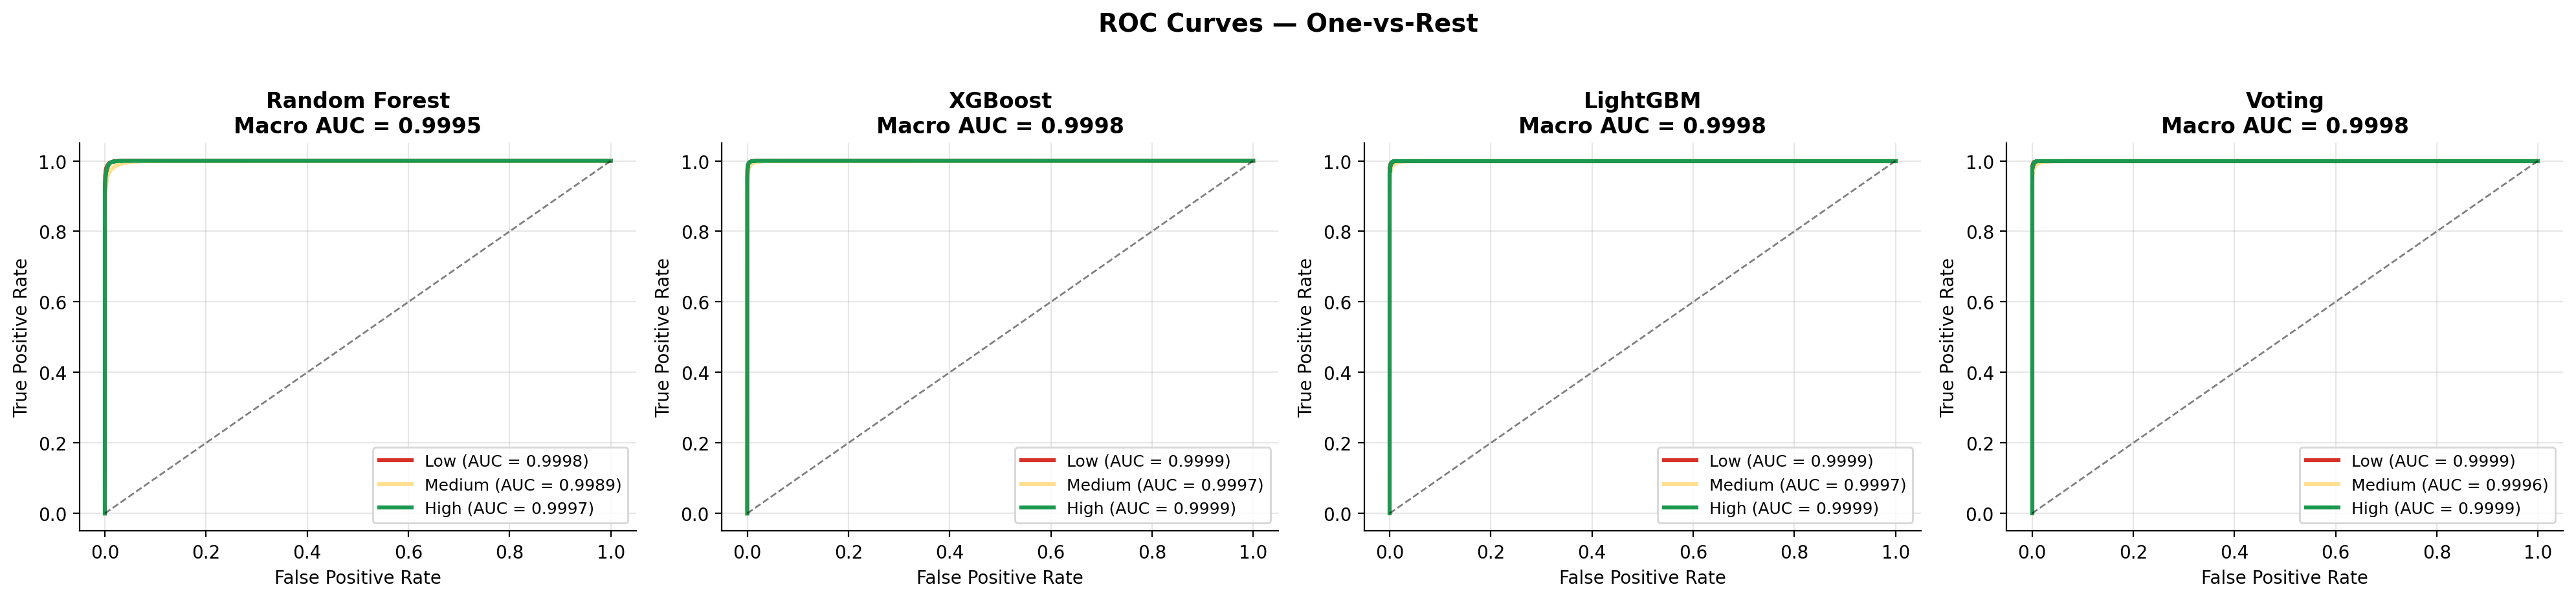
\includegraphics[width=0.78\textwidth]{roc_curves}
  \caption{One-vs-rest ROC curves for the four classifiers on the test set. All
           curves approach the ideal upper-left corner (AUC $\approx 0.9998$).}
  \label{fig:roc}
\end{figure}

\begin{figure}[H]
  \centering
  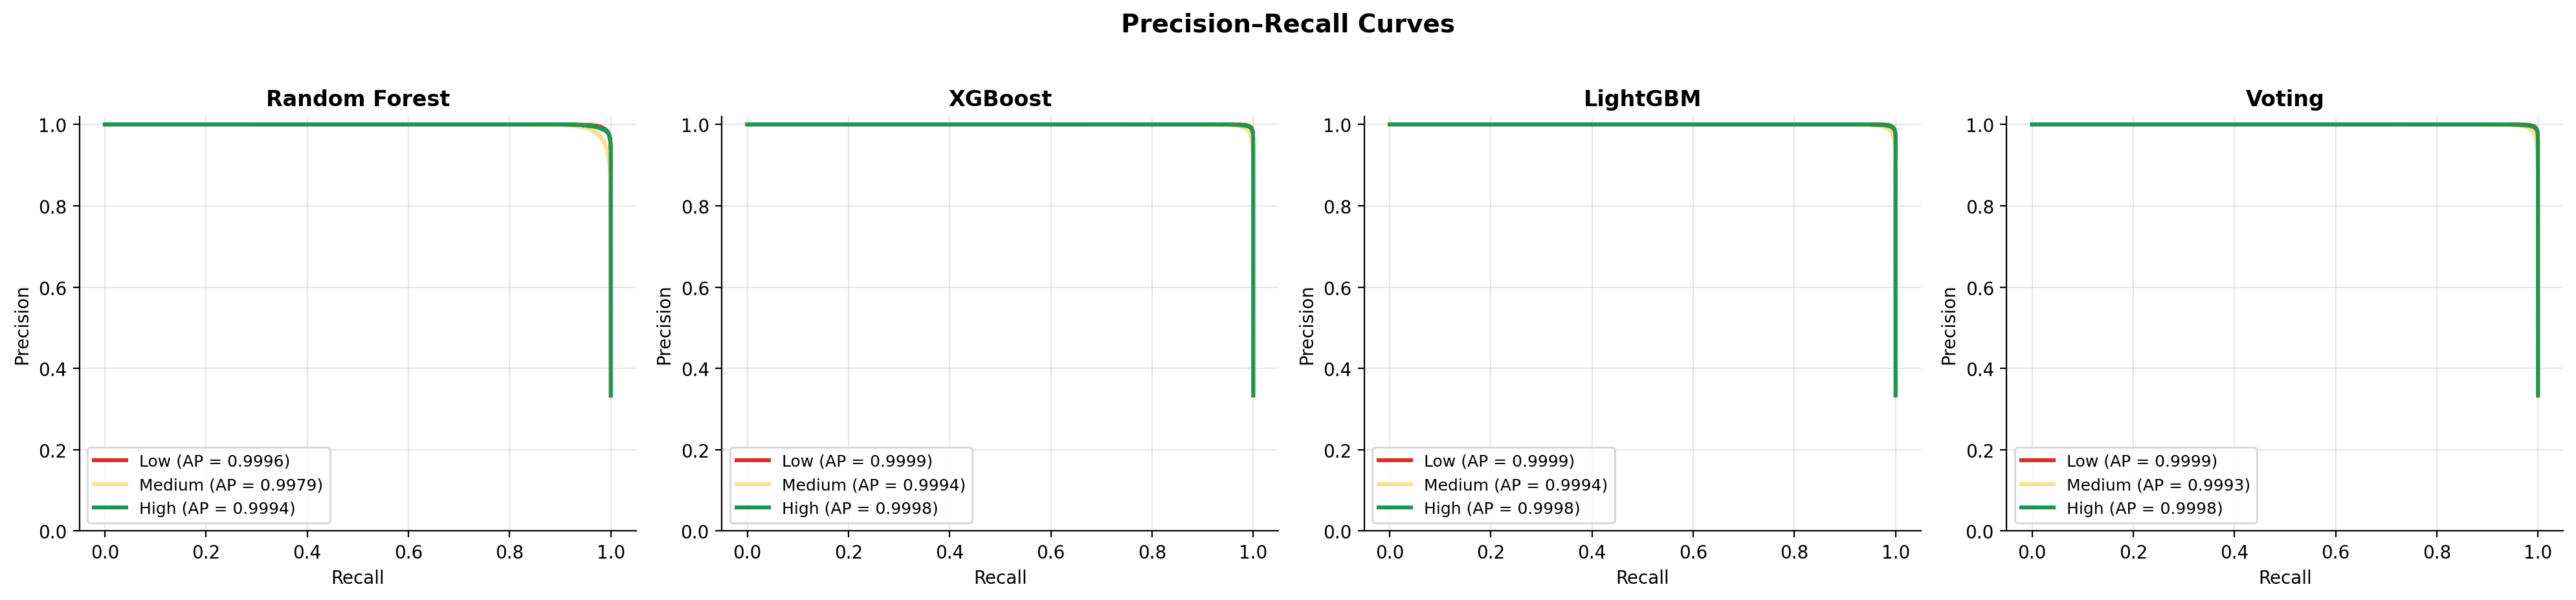
\includegraphics[width=0.78\textwidth]{pr_curves}
  \caption{Precision--recall curves for the three potential classes, confirming
           high precision is maintained across the full recall range.}
  \label{fig:pr}
\end{figure}

\subsection{Cross-Validation}
\label{sec:cv}

To confirm that the test-set performance was not an artefact of one particular
split, each model was also assessed under five-fold cross-validation on the
training data (Table~\ref{tab:cv}). The fold-to-fold variation is very small for
all three tree ensembles---standard deviations of a few ten-thousandths in macro
$F_1$---indicating stable, reproducible performance rather than a fortunate
partition. LightGBM showed the tightest spread, XGBoost the best test-set
metrics; in practice the two are interchangeable on this data, and either would
serve as the production model.

\begin{table}[H]
\centering
\caption{Five-fold cross-validated macro $F_1$ (mean $\pm$ standard deviation)
         on the training set.}
\label{tab:cv}
\begin{tabular}{lc}
\toprule
Model & Macro $F_1$ (mean $\pm$ SD) \\
\midrule
Random Forest & $0.9839 \pm 0.0005$ \\
XGBoost       & $0.9896 \pm 0.0004$ \\
LightGBM      & $0.9911 \pm 0.0002$ \\
\bottomrule
\end{tabular}
\end{table}

\begin{figure}[H]
  \centering
  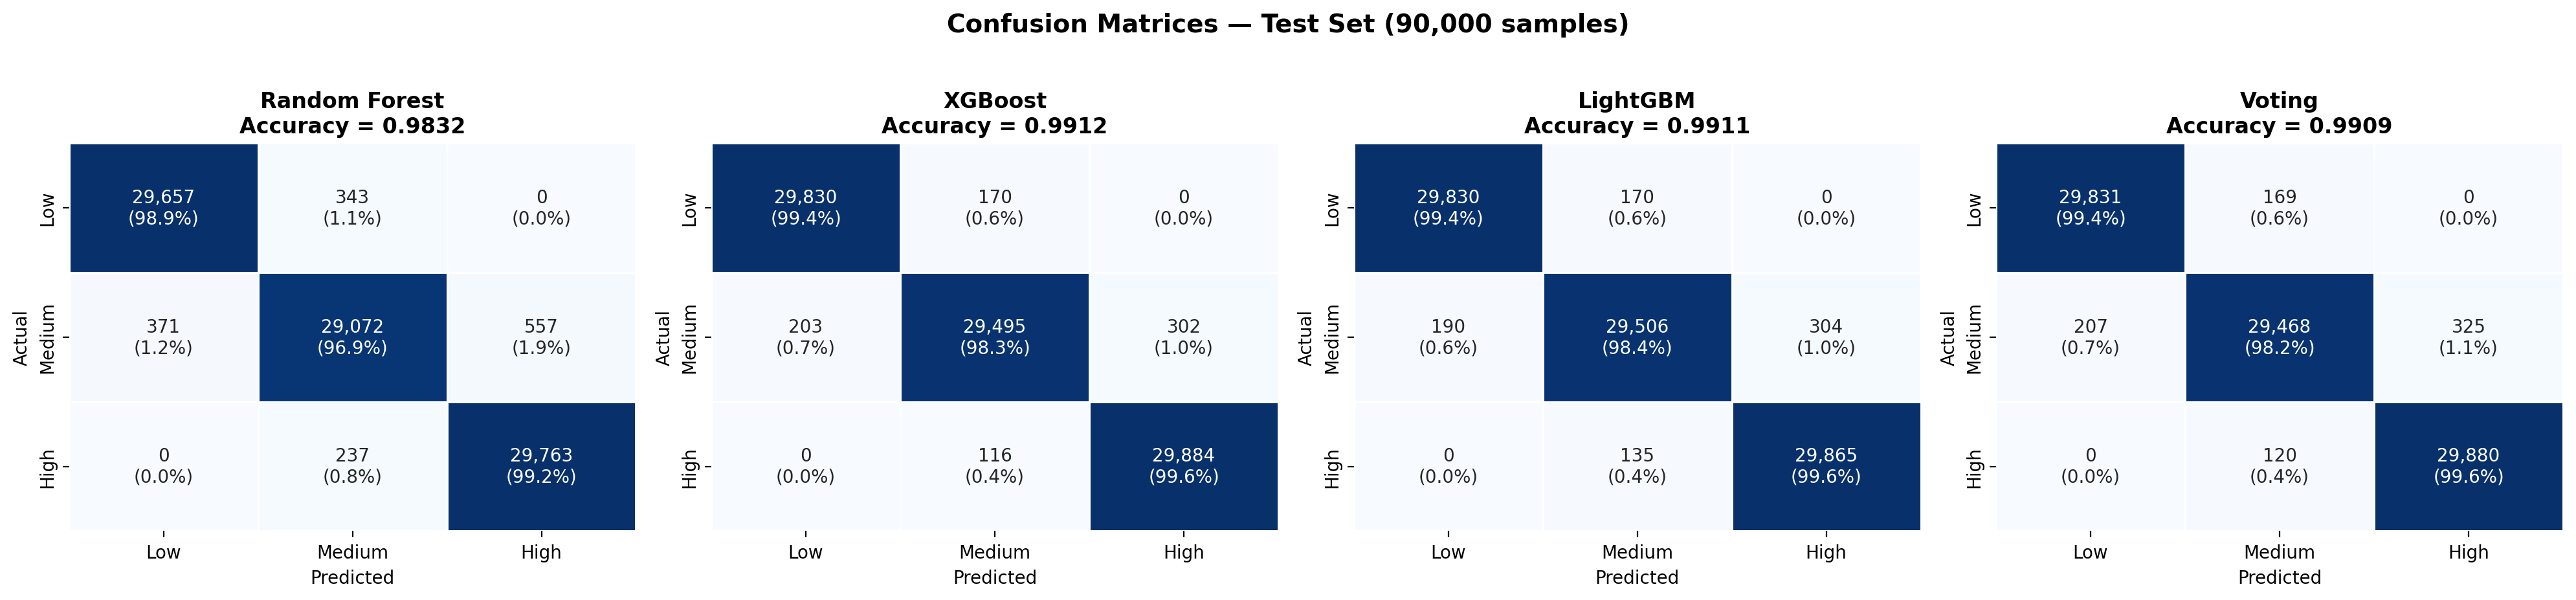
\includegraphics[width=0.8\textwidth]{confusion_matrices}
  \caption{Confusion matrices for the four classifiers on the test set. Almost
           all mass lies on the diagonal; the few off-diagonal errors occur
           between adjacent classes (Low--Medium and Medium--High).}
  \label{fig:confusion}
\end{figure}

The confusion matrices (Figure~\ref{fig:confusion}) make the error structure
explicit: what little misclassification occurs is confined to neighbouring
classes, with essentially no Low pixels mistaken for High or vice versa. For an
ordinal target this is the most benign error pattern possible.

\section{Feature Importance}
\label{sec:feature_importance}

The features the models relied on agree closely with the exploratory correlations.
For both random forest and XGBoost, soil texture was overwhelmingly the most
important predictor, with an XGBoost importance of 0.831; rainfall ranked second
(random forest importance 0.198, LightGBM 0.236). The remaining features carried
modest weight, and LightGBM---consistent with its leaf-wise growth---spread
importance somewhat more evenly than the other two models.
Figure~\ref{fig:feature_importance} shows the comparison.

\begin{figure}[H]
  \centering
  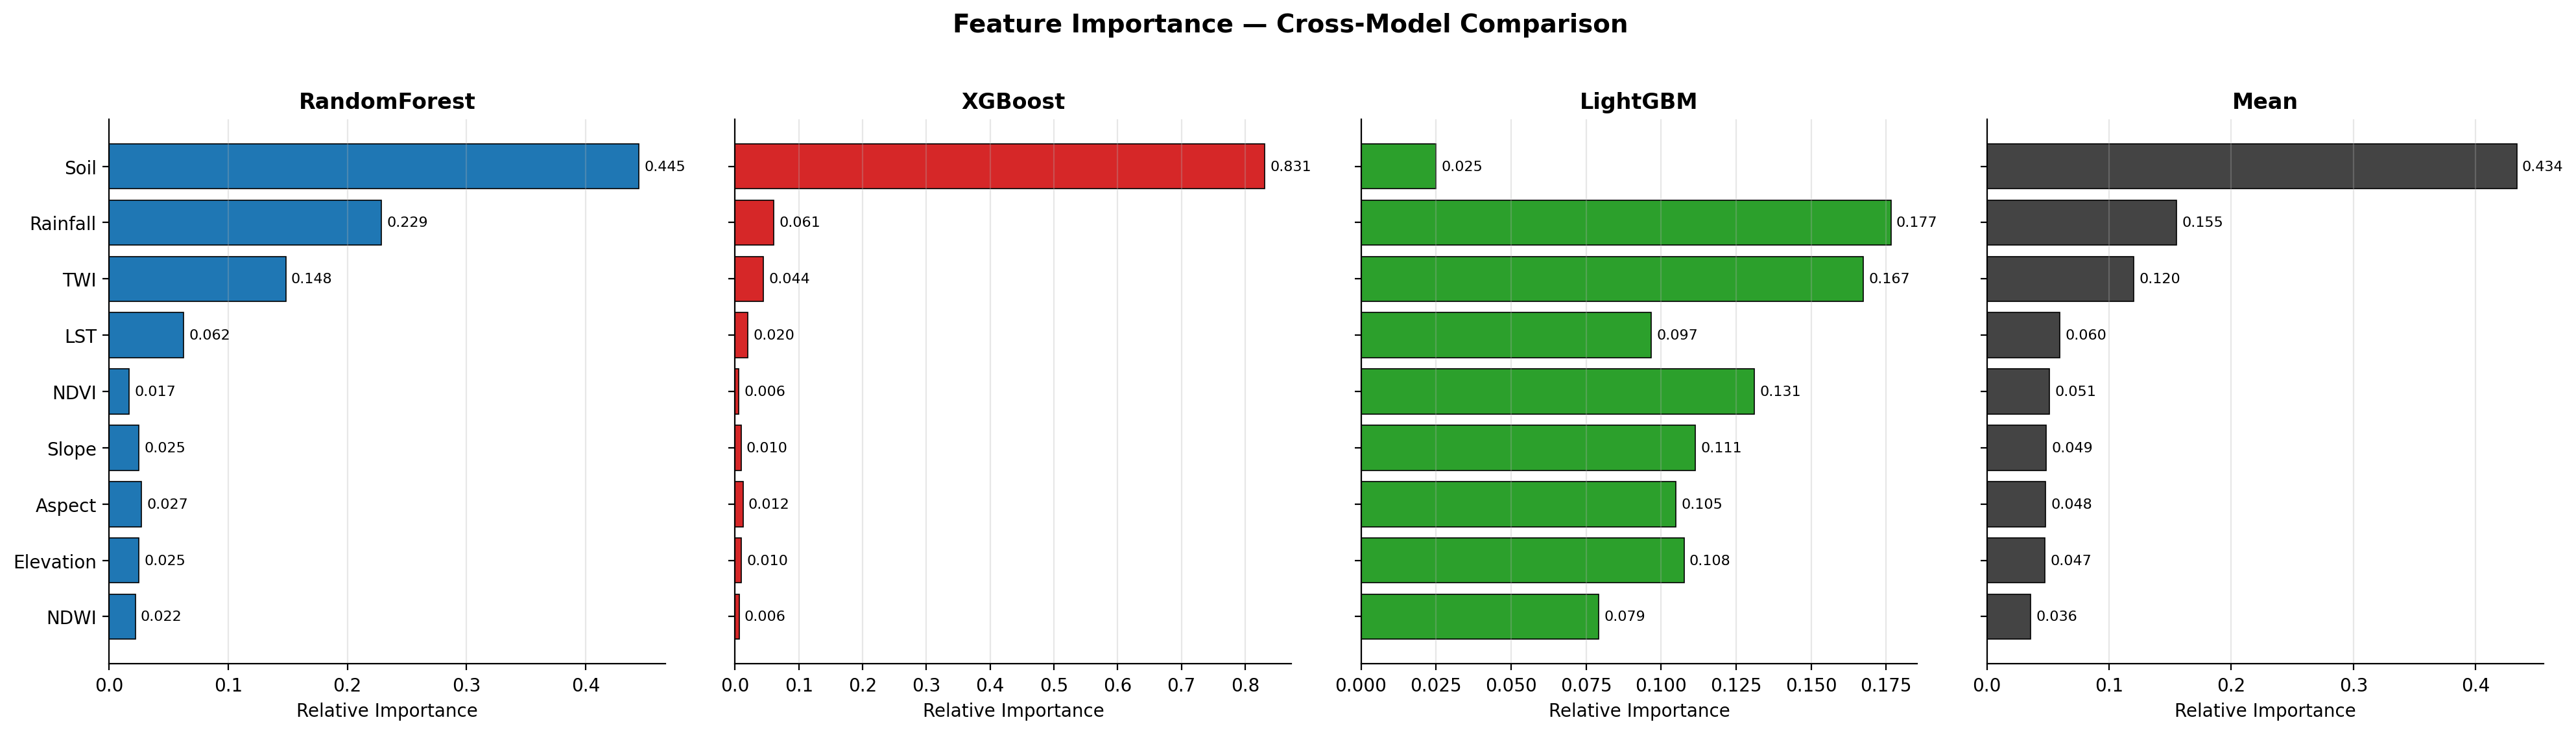
\includegraphics[width=\textwidth]{feature_importance}
  \caption{Feature importance across random forest, XGBoost, and LightGBM. Soil
           texture dominates, with rainfall a consistent second.}
  \label{fig:feature_importance}
\end{figure}

That a learned, nonlinear model independently arrives at the same two dominant
factors as the correlation analysis---soil and rainfall---is reassuring. It also
aligns with the reference study \cite{waqas2022chakwal}, in which geology and
land use (the closest analogues to soil permeability) carried the largest
weights, and it confirms that the model's behaviour is hydrogeologically
sensible rather than being driven by spurious associations.

\section{Groundwater Potential Map}
\label{sec:prediction_map}

Applying the XGBoost model to all \npixels{} valid pixels produced the
full-resolution groundwater potential map in Figure~\ref{fig:gw_map}. The spatial
distribution of the three classes is given in Table~\ref{tab:pixel_dist}.

\begin{table}[H]
\centering
\caption{Predicted groundwater potential distribution across the \studyarea{}.}
\label{tab:pixel_dist}
\begin{tabular}{lcc}
\toprule
Zone & Pixel count & Coverage (\%) \\
\midrule
Low potential    & 14{,}806{,}035 & 40.0 \\
Medium potential & 14{,}806{,}036 & 40.0 \\
High potential   &  7{,}403{,}020 & 20.0 \\
\midrule
\textbf{Total}   & \textbf{\npixels{}} & \textbf{100.0} \\
\bottomrule
\end{tabular}
\end{table}

\begin{figure}[H]
  \centering
  \includegraphics[width=\textwidth]{Fig1_GW_Prediction_Map}
  \caption{Groundwater potential map of the \studyarea{} predicted by XGBoost at
           30~m resolution. High-potential ground (green) concentrates along the
           northern alluvial tracts and major river valleys; low-potential ground
           (red) dominates the southern hard-rock terrain.}
  \label{fig:gw_map}
\end{figure}

The map places high potential where hydrogeology would lead one to expect it:
along the alluvial corridors of the Soan and the river valleys, and across the
wetter northern districts, while the folded and crystalline terrain of the south
and the Salt Range is predominantly Low. The continuous High-probability surface
(Figure~\ref{fig:gw_prob}) conveys the same pattern with its gradations intact,
and is the layer used for the validation in Section~\ref{sec:validation_results}.

\begin{figure}[H]
  \centering
  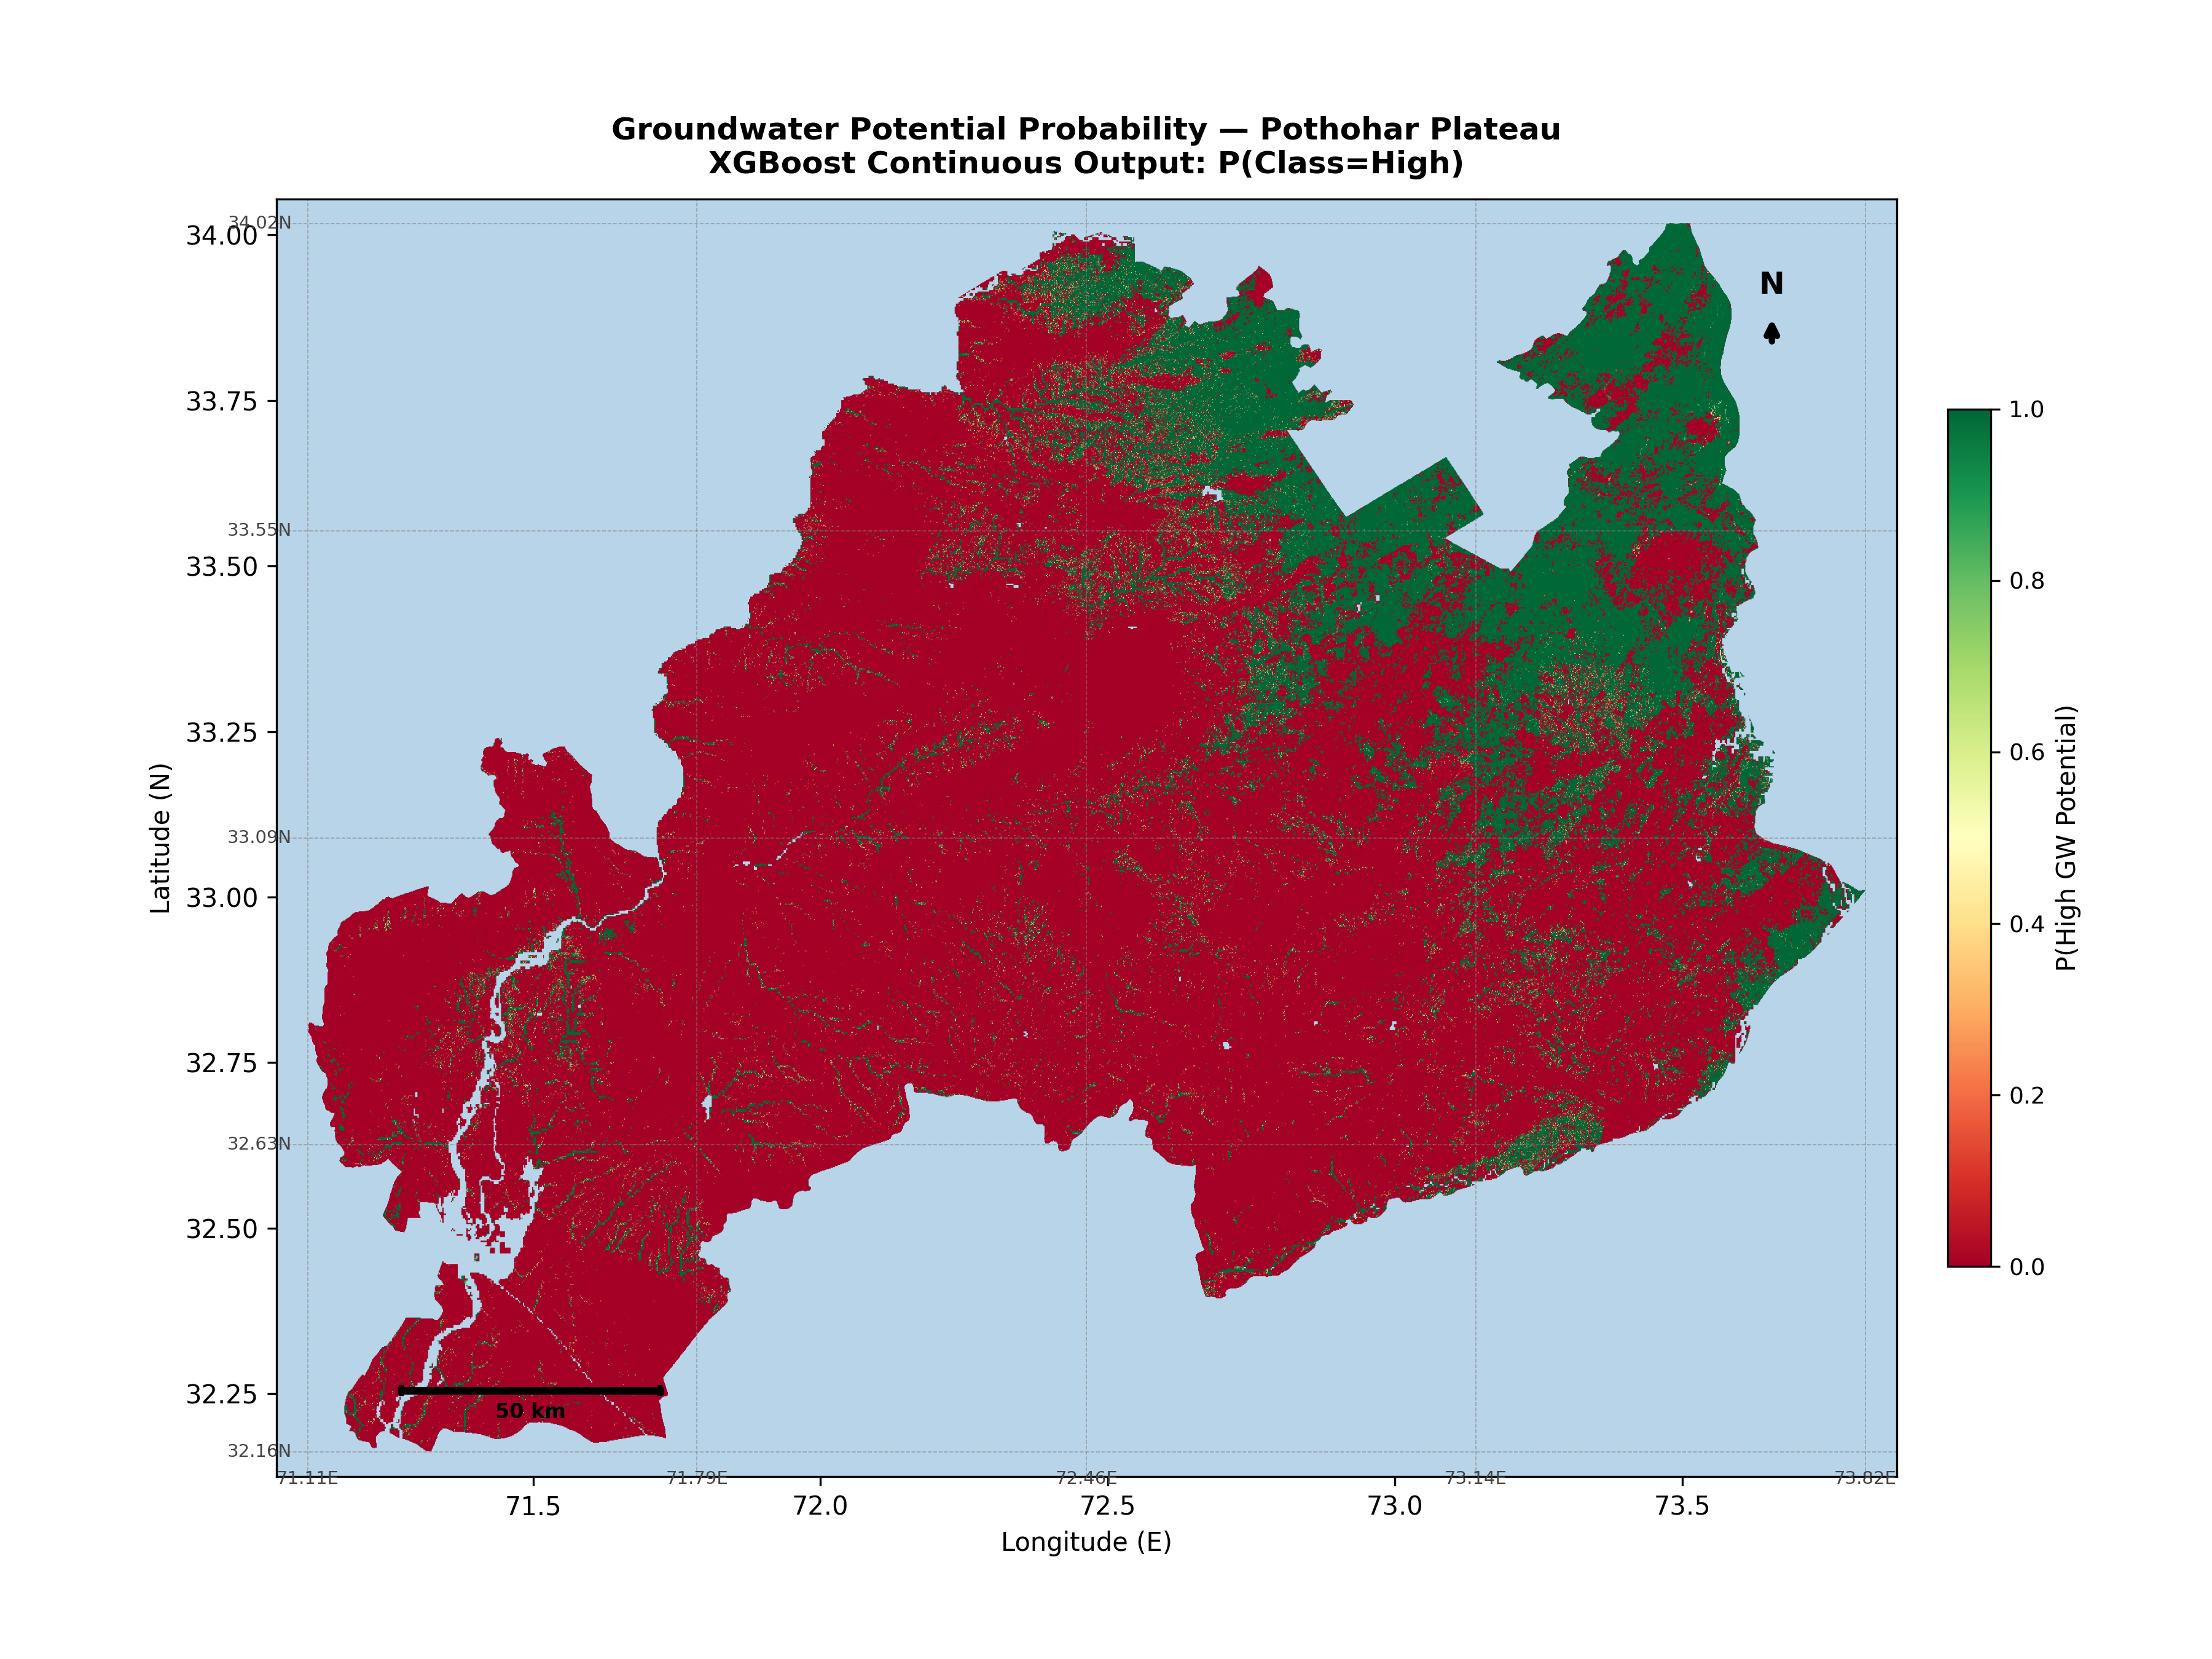
\includegraphics[width=\textwidth]{Fig2_GW_Probability_Map}
  \caption{Continuous probability of the High potential class from the XGBoost
           model, preserving the gradational detail lost in the hard
           classification.}
  \label{fig:gw_prob}
\end{figure}

\subsection{Agreement with the Weighted Overlay}
\label{sec:agreement}

Compared pixel by pixel against the weighted-overlay reference labels across all
37~million valid pixels, the XGBoost map agrees on 99.05\% of them
(Figure~\ref{fig:overlay_compare}). This high agreement is the expected
consequence of training on those labels, and it should be interpreted as evidence
that the model faithfully learned the overlay---not as an independent measure of
correctness. The small disagreements are concentrated, as one would expect, along
the class boundaries where the continuous score crosses a percentile threshold.
Establishing whether the map is correct in a stronger sense requires evidence
external to the labels, which the next section provides.

\begin{figure}[H]
  \centering
  \includegraphics[width=\textwidth]{Fig4_Overlay_vs_ML_Comparison}
  \caption{Side-by-side comparison of the weighted-overlay reference labels and
           the XGBoost prediction, which agree on 99.05\% of the 37~million
           valid pixels.}
  \label{fig:overlay_compare}
\end{figure}

\section{Spatial-Realism Validation}
\label{sec:validation_results}

The four independent checks defined in Section~\ref{sec:validation_design} were
applied to the predicted map. Their combined results are shown in
Figure~\ref{fig:spatial_realism} and described below.

\begin{figure}[H]
  \centering
  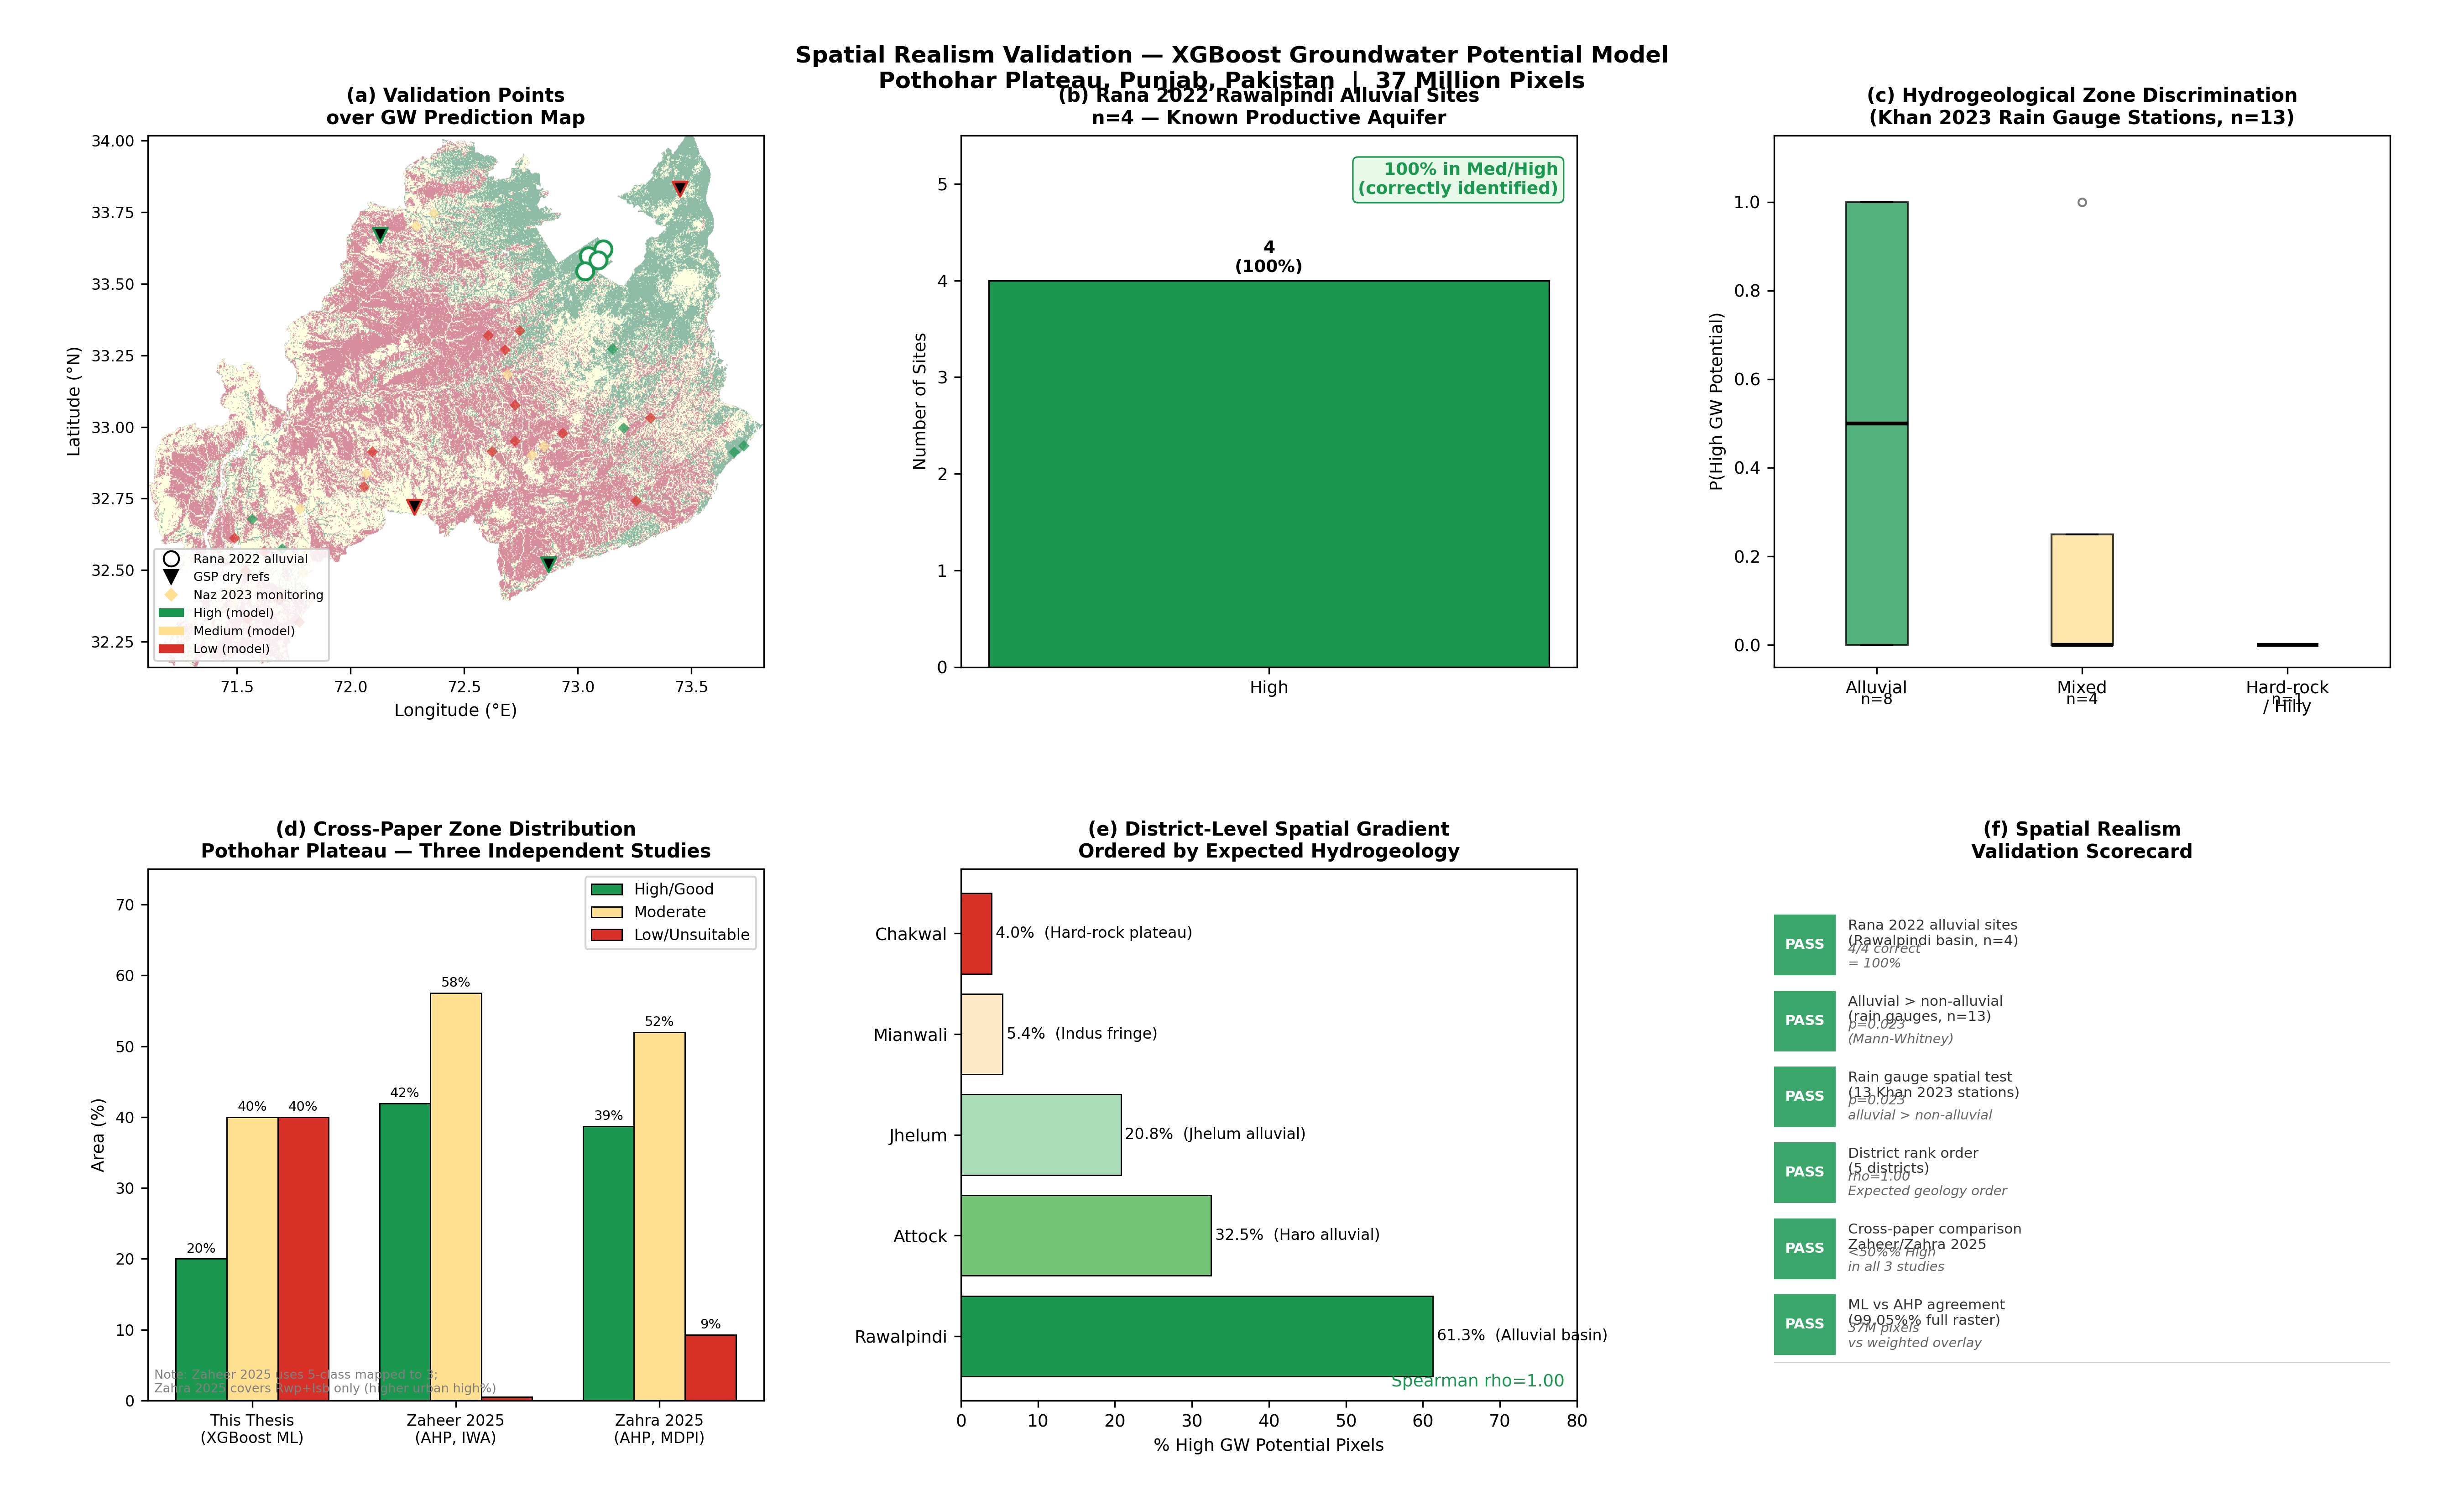
\includegraphics[width=\textwidth]{spatial_realism_validation}
  \caption{Spatial-realism validation summary: (1) known alluvial sites against
           predicted class; (2) recharge-zone discrimination from independent
           rain-gauge stations; (3) cross-study consistency of the
           High-potential fraction; and (4) the district-scale potential
           gradient.}
  \label{fig:spatial_realism}
\end{figure}

\paragraph{Known productive sites.}
All four published groundwater sites in the Rawalpindi alluvial basin fell within
Medium or High potential ground on the predicted map, with High-class
probabilities at or close to one---a 100\% hit rate for locations independently
known to be productive. The number of such sites is small, so this is a
qualitative rather than statistical result, but it is the most direct available
check and the map passes it cleanly.

\paragraph{Recharge-zone discrimination.}
The independent rain-gauge stations of Khan et al.
\cite{khan2023rainfallrunoff}, split into alluvial and non-alluvial groups by
hydrogeological setting, showed a clear separation in predicted potential. The
alluvial stations had a markedly higher predicted High-probability than the
non-alluvial ones, and a one-sided Mann--Whitney $U$ test confirmed the
difference was statistically significant ($p = 0.023$). Because these stations
played no part in training the model, this is genuine external evidence that the
map distinguishes recharge-favourable from recharge-poor ground.

\paragraph{Cross-study consistency.}
The 20\% of the plateau classified as High potential is consistent in magnitude
with independent AHP-based assessments of the same region. Hafeez et al.
\cite{hafeez2025rwh}, mapping water-storage and rainwater-harvesting suitability
across essentially the same districts, identified a minority of the area as most
suitable, in the same broad range. Both approaches agree that high-potential
ground is the exception rather than the rule across this semi-arid upland, which
argues against the prediction being systematically over- or under-stated.

\paragraph{District-scale gradient.}
Ranking the five districts by their predicted fraction of High potential
reproduces the expected hydrogeological order almost exactly. Rawalpindi, the
wettest and most alluvial district, has the largest High fraction at about 61\%,
descending through Attock and Jhelum to Mianwali and Chakwal at only 4--5\%. The
Spearman rank correlation between predicted and expected ordering is
$\rho = 1.00$, a perfect match. This gradient---wet, alluvial north against dry,
hard-rock south---is the single most robust piece of validation evidence,
because it rests on the relative ordering of large district populations rather
than on a handful of points.

\paragraph{Summary.}
Taken together, the four checks point the same way: the map reproduces known
productive ground, separates recharge zones that were never shown to the model,
matches the magnitude of independent regional studies, and follows the expected
district gradient perfectly. None of these tests depends on the weighted-overlay
labels, so they address the credibility question that internal accuracy cannot.
Their interpretation, and the limits of what they can establish, is the subject
of Chapter~\ref{ch:discussion}.

% ============================================================
%  Chapter 5 — Discussion
% ============================================================
\chapter{Discussion}
\label{ch:discussion}

The results of Chapter~\ref{ch:results} raise two distinct questions that are
easily conflated. The first is technical: did the machine-learning models do
what they were asked to do? The second is substantive: is the resulting
groundwater potential map actually useful and correct? Keeping these apart is
essential to an honest reading of this work, and the discussion below is
organized around that distinction---beginning with model behaviour and feature
interpretation, then confronting the label-circularity problem directly, and
finally drawing out what the validation can and cannot establish, how the map
compares with regional studies, where it is likely to be wrong, and what it is
good for.

\section{Model Performance in Context}
\label{sec:discuss_performance}

XGBoost achieved the best results across every metric, though only narrowly ahead
of LightGBM and the voting ensemble. The closeness of the three boosting-based
models is itself informative: when several well-regularized learners converge on
almost identical performance, it usually means they have extracted essentially
all of the available signal, and the remaining differences reflect minor
implementation details rather than any deep advantage. XGBoost's slight edge is
consistent with its regularized objective and column subsampling
\cite{chen2016xgboost}, which tend to help on moderate-dimensional inputs like the
nine-feature stack used here. The ordering---XGBoost first, random forest a clear
step behind---also matches what Sahin \cite{sahin2020ensembletree} found when
comparing the same families for landslide susceptibility, where boosting
outperformed bagging on structurally similar spatial data. That an independent
study on a different hazard reproduces the same ranking gives some confidence that
the result reflects a real property of the methods rather than a quirk of this
dataset.

The absolute numbers, however, demand caution rather than celebration. An accuracy
near 99\% and an AUC of 0.9998 would be extraordinary for a model validated
against field observations; here they are unsurprising, because the target is a
deterministic function of the input features. The next section takes this point
head-on, since it governs how every performance figure in this thesis should be
read.

\section{Feature Importance and Hydrogeology}
\label{sec:discuss_features}

Both the correlation analysis and the trained models identify soil texture and
rainfall as the two controlling factors, and the agreement between a simple linear
diagnostic and a nonlinear ensemble is reassuring. Soil texture's dominance
(XGBoost importance 0.831; $r = 0.836$) is hydrogeologically sensible: texture is
the surface expression of permeability, and permeability decides whether rainfall
infiltrates to recharge an aquifer or runs off. This is also consistent with the
reference study \cite{waqas2022chakwal}, in which geology and land use---the
nearest proxies for subsurface permeability---together carried the largest weight,
and it lends after-the-fact support to the decision to source soil texture from
SoilGrids \cite{poggio2021soilgrids} rather than omit it as the reference study
effectively did.

Rainfall's second place is equally expected in a monsoon-fed, recharge-limited
setting, and it echoes Khan et al. \cite{khan2023rainfallrunoff}, who found
rainfall to be the dominant control on the hydrological response of these same
basins. The near-zero importance of slope ($r = 0.051$) deserves a brief comment
because it might seem to contradict the GWPM literature, where slope is usually a
meaningful factor. The explanation is regional: across a comparatively subdued
plateau, slope varies too little to separate groundwater zones, whereas in the
mountainous catchments where slope is informative the relief is far greater. The
finding is therefore specific to this terrain and should not be generalized.

\section{The Label-Circularity Problem}
\label{sec:discuss_circularity}

The central methodological issue in this work is that the training labels were
generated from the same nine features that the models take as input. The
weighted overlay computes a score from the features, thresholds it into three
classes, and those classes become the targets the models learn to predict. The
consequence is a form of circularity: the models are, in effect, learning to
reproduce a fixed arithmetic combination of their own inputs. The 99.05\%
agreement between the XGBoost map and the overlay labels
(Section~\ref{sec:agreement}), and the near-perfect test metrics, are therefore
largely a measure of how completely the model recovered that combination---not
independent evidence that the map matches real groundwater.

It would be dishonest to present the high accuracy as though it validated the map
against reality, and this thesis does not. What the accuracy does establish is
worth stating precisely, because it is not nothing. It shows that a single learned
model can reproduce the weighted overlay across 37~million pixels faithfully and
efficiently, which means the overlay can be replaced by a model that, unlike the
overlay, does not require fixed expert weights, can represent nonlinear
interactions among features, and yields a continuous probability surface rather
than a hard class. In other words, the contribution of the ML step is not a more
accurate map than the overlay---by construction it is almost the same map---but a
more flexible, reproducible, and extensible way of producing it. This is the same
logic under which knowledge-driven labels have been used to train spatial models
elsewhere; Roy and Saha \cite{roy2019knowledgedriven}, for instance, trained on
expert-weighted targets and treated the exercise as legitimate precisely because
the weighted product encodes real domain knowledge.

The honest conclusion is that internal accuracy cannot certify the map, and a
different kind of evidence is needed. That is the purpose of the spatial-realism
validation, discussed next.

\section{What the Validation Establishes---and What It Does Not}
\label{sec:discuss_validation}

The four checks in Section~\ref{sec:validation_results} were designed to test the
map against evidence that played no part in its construction, and on their own
terms they are encouraging. The map places all four known alluvial sites in
Medium or High ground; it separates independent rain-gauge stations by
hydrogeological setting at a statistically significant level (Mann--Whitney
$p = 0.023$); its 20\% High fraction matches the magnitude of an independent
regional AHP study; and it reproduces the expected district gradient perfectly
(Spearman $\rho = 1.00$). Crucially, none of these uses the overlay labels, so
together they speak to the substantive question that internal accuracy cannot.

Their limits should be stated just as plainly. The known-sites check rests on only
four points and is qualitative. The rain-gauge test, though significant, is based
on a modest number of stations. The cross-study comparison establishes consistency
of magnitude, not agreement pixel by pixel. And the district gradient, while the
strongest of the four because it aggregates large populations, confirms only that
the broad north--south ordering is right, not that any particular hectare is
correctly classified. What the validation supports, then, is a measured claim: the
map is spatially realistic---it is right in its large-scale structure and on the
independent points available---rather than a claim that it is accurate everywhere.
For a data-scarce region this is, realistically, the strongest validation the
available evidence will bear, and it is a more honest position than leaning on the
99\% figure. The recurring difficulty of obtaining adequate ground truth for
groundwater models is itself well documented \cite{hai2022gwlreview}; this thesis
does not escape it, but it does try to be candid about it.

\section{Comparison with the Reference and Regional Studies}
\label{sec:discuss_comparison}

Set against the reference study of Waqas et al. \cite{waqas2022chakwal}, the
advance here is one of scope and method rather than of validated accuracy
(Table~\ref{tab:comparison}). The present work covers all five districts of the
plateau instead of one, uses nine features instead of five, replaces manual
overlay with a learned model, and reports quantitative performance and an
independent validation where the reference study reported neither. These are real
improvements in reproducibility and coverage, and they are the substantive
contribution; the headline accuracy, as discussed, is not directly comparable
because the reference study did not train on its own overlay.

\begin{table}[H]
\centering
\caption{Comparison of this thesis with the reference study of Waqas et al.
         \cite{waqas2022chakwal}.}
\label{tab:comparison}
\small
\begin{tabular}{lll}
\toprule
Aspect & Waqas et al.\ (2022) & This thesis \\
\midrule
Study area & Chakwal (1 district) & Full plateau (5 districts) \\
Method     & Manual weighted overlay & ML (RF, XGBoost, LightGBM, ensemble) \\
Features   & 5 & 9 \\
Validation & Secondary data only & 5-fold CV + spatial-realism checks \\
Output     & Static maps & GeoTIFF class + probability rasters \\
Resolution & Not specified & 30~m \\
\bottomrule
\end{tabular}
\end{table}

The map also sits comfortably alongside other recent work on the region. Hafeez et
al. \cite{hafeez2025rwh}, mapping rainwater-harvesting suitability across
essentially the same districts by AHP, identify a similar minority of the area as
most favourable and locate it in the same alluvial tracts, which is the
cross-study consistency reported in Section~\ref{sec:validation_results}. The
broader move from knowledge-driven overlay to data-driven prediction that this
thesis carries out for groundwater has already been found beneficial for related
problems---Arabameri et al. \cite{arabameri2018shahroud}, comparing approaches on
a single plain, reported data-driven methods matching or exceeding multi-criteria
ones---so the methodological direction taken here is well supported even if the
circularity caveat tempers the accuracy gain.

\section{Likely Errors: Hard-Rock Terrain and the Missing Lithology Layer}
\label{sec:discuss_hardrock}

The clearest weakness of the map is expected to lie in the hard-rock uplands. The
nine features capture surface and climatic conditions well, but they say nothing
direct about subsurface lithology or fracturing, and in crystalline or massively
bedded terrain these are precisely the controls that matter. Benjmel et al.
\cite{benjmel2020morocco} showed that in such settings lineament density and
geological structure dominate groundwater occurrence, with fracture zones acting
as conduits through otherwise impermeable rock. Where parts of the Margalla Hills
or the Kala Chitta Range carry high rainfall and dense vegetation, the model is
liable to read those surface signals as high potential even though the underlying
rock may store little water. The absence of a lithological or lineament layer is
thus the most probable source of systematic over-prediction, and adding a
digitized geological map---from Geological Survey of Pakistan sheets---as a tenth
feature is the single most valuable improvement available to future work.

A second, subtler caveat concerns the distinction between potential and
potability. The model predicts where groundwater is likely to occur, not whether
it is fit to use. In the peri-urban Rawalpindi--Islamabad belt, shallow aquifers
carry a documented contamination risk \cite{waseem2024waterquality}, so a
high-potential classification there should be read as "water is likely present,"
not "water is safe to drink." A water-quality layer would be needed to bridge that
gap.

\section{Practical Implications}
\label{sec:discuss_implications}

With those caveats in mind, the map still carries practical value for an area
where groundwater siting is currently done with little spatial guidance. The High
potential zone---about 20\% of the plateau, on the order of a few thousand square
kilometres---is concentrated along the Soan basin and the northern and riverine
alluvial corridors, and these are the natural first places to consider for new
wells or managed recharge. The Low zone, dominating the southern hard-rock
terrain, flags where deep borehole investment is least likely to pay off, subject
to the lithology caveat above. Because the outputs are standard GeoTIFF rasters at
30~m resolution---both a hard classification and a continuous probability
surface---they can be brought directly into the GIS workflows of agencies such as
PCRWR and the provincial irrigation department for district-level planning. In a
region where rain-fed agriculture leaves households acutely dependent on
groundwater through the dry season \cite{sarwar2022soandrought}, even a
spatially-realistic first-order map is more useful than none.

\section{Limitations}
\label{sec:discuss_limitations}

Several limitations have been noted in passing and are collected here for clarity.
The foremost is label circularity: with no plateau-wide field measurements, the
models were trained on knowledge-based labels, so internal accuracy measures
fidelity to the overlay rather than to ground truth. The validation, while
independent, rests on relatively few points and establishes spatial realism rather
than pixel-level accuracy. The feature set omits subsurface lithology and
lineaments, which likely causes over-prediction in hard-rock zones, and it
includes no water-quality information. Finally, the static input layers---a
multi-year rainfall sum, single-period spectral indices---describe an average
condition and do not capture seasonal or interannual variation in groundwater.
None of these undermines the central contribution, but each marks a place where
the map should be used with appropriate caution and where future work can
strengthen it.

% ============================================================
%  Chapter 6 — Conclusion
% ============================================================
\chapter{Conclusion and Future Work}
\label{ch:conclusion}

\section{Summary of the Study}
\label{sec:concl_summary}

This thesis set out to bring groundwater potential mapping of the \studyarea{}
from a single district and a manual method up to the full five-district plateau
and a machine-learning method. Nine geo-environmental features---elevation,
slope, aspect, topographic wetness index, NDVI, NDWI, rainfall, soil texture, and
land surface temperature---were assembled at 30~m resolution through Google Earth
Engine for the whole of Chakwal, Rawalpindi, Attock, Jhelum, and Mianwali,
yielding \npixels{} valid pixels. A knowledge-based weighted overlay supplied
three-class reference labels, a balanced sample of 450,000 pixels was used to
train four classifiers, and the best of these was applied across the plateau to
produce a full-resolution map, which was then tested against independent evidence.
The work thereby answers the four research questions posed in
Chapter~\ref{ch:introduction}, as summarized below.

\section{Key Findings}
\label{sec:concl_findings}

\begin{itemize}
  \item \textbf{Reproducing and refining the overlay (RQ1).} A single XGBoost
        model reproduced the knowledge-based weighted overlay across all
        37~million pixels with 99.05\% agreement, confirming that supervised
        learning can stand in for the manual method---while doing so in a form
        that needs no fixed expert weights and yields a continuous probability
        surface.

  \item \textbf{Best model (RQ2).} Of the four classifiers, XGBoost performed best
        on every metric (99.12\% accuracy, macro $F_1 = 0.991$, Cohen's
        $\kappa = 0.987$, ROC-AUC $= 0.9998$), narrowly ahead of LightGBM and the
        voting ensemble and a clear step above random forest. The differences
        among the boosting models are small enough that any of them would serve in
        practice.

  \item \textbf{Controlling factors (RQ3).} Soil texture ($r = 0.836$; XGBoost
        importance 0.831) and rainfall ($r = 0.514$) emerged as the dominant
        predictors from both the correlation analysis and the trained models,
        consistent with the hydrogeology of a semi-arid, recharge-limited plateau
        and with the reference study's emphasis on permeability-related factors.

  \item \textbf{Independent credibility (RQ4).} A spatial-realism validation, using
        evidence that played no part in training, supported the map on all four
        checks: known alluvial sites fell in Medium or High ground, independent
        rain-gauge stations separated by hydrogeological setting at a significant
        level ($p = 0.023$), the 20\% High fraction matched independent regional
        AHP work, and the district-scale potential gradient reproduced the expected
        north--south ordering exactly ($\rho = 1.00$).
\end{itemize}

Across the plateau the model classified 20\% of the area as High potential, 40\%
as Medium, and 40\% as Low, with high potential concentrated along the Soan basin
and the northern and riverine alluvial corridors.

\section{Contributions}
\label{sec:concl_contributions}

The study delivers the first machine-learning groundwater potential map of the
full \studyarea{} at 30~m resolution, expanding the feature set of the reference
study from five layers to nine, providing a systematic comparison of four
classifiers on a balanced dataset, and---perhaps most importantly for a
data-scarce region---demonstrating a transparent, evidence-based way to validate
such a map when field measurements are unavailable. The accompanying GeoTIFF
outputs, both a hard classification and a continuous probability surface, are
directly usable in the GIS workflows of regional water-resource agencies.

\section{Limitations}
\label{sec:concl_limitations}

The findings should be read with the limitations set out in
Chapter~\ref{ch:discussion}. Chief among them is label circularity: because the
training labels were derived from the same features used as inputs, the high
internal accuracy measures fidelity to the weighted overlay rather than to ground
truth, and the map's real-world credibility rests on the spatial-realism
validation rather than on its accuracy figures. The validation, though
independent, is built on relatively few points and establishes large-scale
realism rather than pixel-level correctness. The feature set omits subsurface
lithology and lineaments---likely causing over-prediction in hard-rock terrain---
as well as water-quality information, and its static layers describe an average
rather than a time-varying condition.

\section{Recommendations for Future Work}
\label{sec:concl_future}

Several extensions follow naturally and would strengthen the map in roughly this
order of priority.

\begin{enumerate}
  \item \textbf{Add a lithological layer.} Digitizing geological and lineament
        information from Geological Survey of Pakistan sheets and adding it as a
        tenth feature is the single most valuable improvement. It would directly
        address the expected over-prediction in the crystalline and folded terrain
        of the Salt Range, Margalla Hills, and Kala Chitta Range, where structure
        rather than surface condition governs groundwater \cite{benjmel2020morocco}.

  \item \textbf{Incorporate field-measured well data.} Where borehole yield or
        water-level records can be obtained---for example through the PCRWR
        monitoring network---they would allow a true accuracy assessment to
        complement, and eventually move beyond, the knowledge-based labels,
        loosening the circularity that constrains the present interpretation.

  \item \textbf{Add a water-quality dimension.} A contamination or salinity layer
        would let the map distinguish high-potential ground that is fit for use
        from high-potential ground that is not, a distinction that matters
        particularly in the peri-urban Rawalpindi belt \cite{waseem2024waterquality}.

  \item \textbf{Capture temporal dynamics.} Replacing the static rainfall and
        spectral summaries with multi-temporal inputs would allow seasonal and
        interannual variation in recharge to be represented, rather than a single
        average condition.

  \item \textbf{Deliver an interactive product.} Publishing the map as a web-based
        GIS layer would put it directly in the hands of district planners and
        farmers, turning a research output into a usable decision-support tool.
\end{enumerate}

\section{Concluding Remarks}
\label{sec:concl_remarks}

Groundwater will only become more central to the \studyarea{} as rainfall grows
less reliable and demand continues to rise, a pressure visible across aquifers
worldwide \cite{jasechko2024gwdecline}. Knowing where the resource is likely to be
found is a precondition for managing it well. This thesis has shown that machine
learning can take over the mapping task from manual weighted overlay across the
whole plateau, at fine resolution, and---when its limitations are acknowledged
rather than hidden---can be validated against independent hydrogeological evidence
rather than internal accuracy alone. The result is not a final answer but a
defensible and extensible foundation: a first regional, reproducible groundwater
potential map for the \studyarea{}, and a clear path, beginning with the addition
of subsurface geology, toward making it better.


% ---------------- References --------------------------------
\cleardoublepage
\addcontentsline{toc}{chapter}{References}
\bibliography{references}

% ---------------- Appendices --------------------------------
\appendix
% ============================================================
%  Appendix A — Implementation and Code
% ============================================================
\chapter{Implementation and Code}
\label{app:code}

This appendix documents the software implementation of the analysis. The full
pipeline was written in Python~3.13 and organized as a sequence of scripts, each
corresponding to one stage of the workflow in Chapter~\ref{ch:methodology}.

\section{Software Environment}
\label{app:env}

The principal libraries used were \texttt{earthengine-api} and \texttt{geemap}
for data collection; \texttt{rasterio} and \texttt{geopandas} for geospatial
preprocessing; \texttt{numpy} and \texttt{pandas} for array and table handling;
and \texttt{scikit-learn}, \texttt{xgboost}, and \texttt{lightgbm} for model
training and evaluation. Figures were produced with \texttt{matplotlib} and
\texttt{contextily}.

\section{Pipeline Scripts}
\label{app:scripts}

Table~\ref{tab:scripts} lists the scripts in execution order and the role of each.

\begin{table}[H]
\centering
\caption{Pipeline scripts in execution order.}
\label{tab:scripts}
\small
\begin{tabular}{p{4.4cm} p{8.6cm}}
\toprule
Script & Function \\
\midrule
\texttt{collect\_data.py}        & Assemble the nine features in Google Earth Engine and export the multi-band GeoTIFF. \\
\texttt{preprocess.py}           & Mask to district boundaries, min--max normalize each band, quality-check. \\
\texttt{step1\_generate\_labels.py} & Weighted-overlay scoring and percentile thresholding into three classes. \\
\texttt{step2\_validate.py}      & Exploratory analysis: correlations, distributions, class balance. \\
\texttt{step3\_train\_models.py} & Train and evaluate RF, XGBoost, LightGBM, and the voting ensemble; 5-fold CV. \\
\texttt{step4\_predict\_map.py}  & Tiled full-plateau prediction; classified and probability rasters. \\
\texttt{step9\_spatial\_realism\_validation.py} & The four spatial-realism checks and summary figure. \\
\bottomrule
\end{tabular}
\end{table}

\section{Representative Code}
\label{app:snippets}

The weighted-overlay score that produced the training labels
(Equation~\ref{eq:overlay}) was implemented as a direct weighted sum of the
normalized bands, with negatively-related features inverted before weighting:

\begin{verbatim}
# Weighted overlay: composite groundwater potential score
weights = {
    'soil': 0.25, 'twi': 0.20, 'rainfall': 0.20, 'ndvi': 0.10,
    'slope': 0.10, 'ndwi': 0.05, 'elevation': 0.05, 'lst': 0.03,
    'aspect': 0.02,
}
invert = {'slope', 'elevation', 'lst'}   # higher value -> lower potential

score = np.zeros(n_pixels, dtype=np.float32)
for name, w in weights.items():
    f = bands[name]                      # normalized to [0, 1]
    score += w * (1.0 - f if name in invert else f)

# Percentile thresholds: 40% Low, 40% Medium, 20% High
low_t, high_t = np.percentile(score, [40, 80])
labels = np.where(score < low_t, 0, np.where(score < high_t, 1, 2))
\end{verbatim}

The XGBoost classifier was configured with the hyperparameters reported in
Section~\ref{sec:ml_models}:

\begin{verbatim}
from xgboost import XGBClassifier

model = XGBClassifier(
    n_estimators=300,
    learning_rate=0.1,
    max_depth=6,
    subsample=0.8,
    colsample_bytree=0.8,
    objective='multi:softprob',
    num_class=3,
    n_jobs=-1,
)
model.fit(X_train, y_train)
\end{verbatim}

Full-plateau prediction was carried out over $2048 \times 2048$ pixel tiles to
keep memory use bounded, with each tile classified and written back to the output
raster before the next was read.

% ============================================================
%  Appendix B — Data Sources and Outputs
% ============================================================
\chapter{Data Sources and Outputs}
\label{app:data}

\section{Source Datasets}
\label{app:sources}

All input data were obtained through Google Earth Engine. Table~\ref{tab:gee_full}
gives the full dataset identifiers, native resolutions, and the temporal windows
used.

\begin{table}[H]
\centering
\caption{Google Earth Engine source datasets for the nine input features.}
\label{tab:gee_full}
\small
\begin{tabular}{p{2.3cm} p{5.4cm} p{2.2cm} p{2.6cm}}
\toprule
Feature & GEE dataset & Native res. & Period \\
\midrule
Elevation & \texttt{USGS/SRTMGL1\_003} & 30~m & 2000 \\
Slope, Aspect & \texttt{ee.Terrain} (from SRTM) & 30~m & 2000 \\
TWI & \texttt{WWF/HydroSHEDS/15ACC} + SRTM & 15~arc-sec & static \\
NDVI, NDWI & \texttt{LANDSAT/LC08/C02/T1\_L2} & 30~m & 2015--2023 \\
Rainfall & \texttt{UCSB-CHG/CHIRPS/DAILY} & 0.05$^\circ$ & 2015--2023 \\
Soil texture & \texttt{OpenLandMap/SOL/SOL\_TEXTURE-CLASS\_USDA-TT\_M/v02} & 250~m & static \\
LST & \texttt{MODIS/061/MOD11A1} & 1~km & 2015--2023 \\
\bottomrule
\end{tabular}
\end{table}

All bands were resampled to a common 30~m grid in EPSG:4326 on export, and
reprojected to UTM Zone~42N (EPSG:32642) for area and distance calculations. The
exported raster is $10{,}062 \times 6{,}884$ pixels (about 69.2~million cells), of
which \npixels{} (53.4\%) lie within the five district boundaries and carry valid
data.

\section{Study Area Specification}
\label{app:area}

\begin{table}[H]
\centering
\caption{Study area parameters.}
\label{tab:area_spec}
\begin{tabular}{ll}
\toprule
Parameter & Value \\
\midrule
Districts & Chakwal, Rawalpindi, Attock, Jhelum, Mianwali \\
Approx.\ area & \SI{25000}{\kilo\meter\squared} \\
Latitude range & \ang{32.16}--\ang{34.02}~N \\
Longitude range & \ang{71.11}--\ang{73.82}~E \\
Export CRS & EPSG:4326 \\
Analysis CRS & EPSG:32642 (UTM Zone 42N) \\
Resolution & 30~m \\
Valid pixels & \npixels{} \\
\bottomrule
\end{tabular}
\end{table}

\section{Model Outputs}
\label{app:outputs}

The principal geospatial outputs of the study are listed in
Table~\ref{tab:outputs}. The classified and probability rasters are the
deliverables intended for downstream GIS use.

\begin{table}[H]
\centering
\caption{Principal model outputs.}
\label{tab:outputs}
\small
\begin{tabular}{p{5.2cm} p{8cm}}
\toprule
Output & Description \\
\midrule
\texttt{gw\_prediction\_xgboost.tif} & Classified groundwater potential (0 = Low, 1 = Medium, 2 = High), 30~m. \\
\texttt{gw\_probability\_high.tif}   & Continuous probability of the High class, 30~m. \\
\texttt{gw\_potential\_labels.tif}   & Weighted-overlay reference labels. \\
\texttt{best\_model.joblib}          & Trained XGBoost model. \\
\texttt{metrics.json}                & Full accuracy report and per-class metrics. \\
\bottomrule
\end{tabular}
\end{table}

\section{Predicted Distribution by District}
\label{app:district}

Table~\ref{tab:district_high} reports the share of each district classified as
High potential, which forms the basis of the district-gradient validation in
Section~\ref{sec:validation_results}. The ordering follows the expected
hydrogeological gradient from the wetter, alluvial north to the drier, hard-rock
south (Spearman $\rho = 1.00$).

\begin{table}[H]
\centering
\caption{Predicted High-potential fraction by district.}
\label{tab:district_high}
\begin{tabular}{lc}
\toprule
District & High potential (\%) \\
\midrule
Rawalpindi & 61.3 \\
Attock     & 32.5 \\
Jhelum     & 20.8 \\
Mianwali   & 5.4 \\
Chakwal    & 4.0 \\
\bottomrule
\end{tabular}
\end{table}


\end{document}
